%!TeX root = BasiDiDati.tex

\chapter{Strutture fisiche e di accesso ai dati}
Le basi di dati risiedono nella \textcolor{azzurrino}{\textbf{memoria secondaria}} perchè sono:
\begin{itemize}[label=$\triangleright$, itemsep=\smallskipamount]
  \item \textbf{grandi}: non possono essere contenute completamente in memoria centrale
  \smallskip
  \item \textbf{persistenti}: hanno un tempo di vita che non è limitato all'esecuzione dei programmi che le usano
\end{itemize}

\vario{Caratteristiche della memoria secondaria}{
  Le caratteristiche principali della memoria secondaria sono:
  \begin{itemize}[label=$\circ$, itemsep=\smallskipamount]
    \item \textbf{non utilizzabile direttamente dai programmi}
    \item \textbf{dati organizzati in blocchi} (grandezza dipende dal sistema operativo)
    \item \textbf{operazioni possibili}:
    \begin{itemize}[label=$\diamond$]
      \item lettura intero blocco
      \item scrittura intero blocco
    \end{itemize}
    \item \textbf{costo delle operazioni di accesso alla memoria secondaria è maggiore al costo per accedere ai dati in memoria centrale}
  \end{itemize}
}

\section{Gestore del buffer}
L'interazione tra memoria secondaria e memoria centrale avviene tramite il \textcolor{azzurrino}{\textbf{gestore del buffer}}, mediante il trasferimento di uno o più \textbf{blocchi} della memoria secondaria in \textbf{pagine} dedicate della memoria centrale (buffer).

\vario{Precisazione}{
  La dimensione delle pagine in memoria centrale sono solitamente un multiplo della dimensione dei blocchi in memoria secondaria.

  \smallskip
  Per semplificare, si assume che siano uguali:
  \begin{equation*}
    \text{1 pagina} \approx \text{1 blocco}
  \end{equation*}
}

\subsection{Buffer}
Il \textcolor{azzurrino}{\textbf{buffer}} è una zona della memoria condivisa dalle applicazioni e una gestione ottimale del buffer consente di ottenere buone prestazioni nell'accesso ai dati.\\[0.2ex]
Quando uno stesso dato viene utilizzato più volte in tempi ravvicinati il buffer evita
l'accesso alla memoria secondaria.

\vario{Compito del gestore del buffer}{
  Il gestore del buffer si occupa di caricare e salvare i dati dalla memoria secondaria alla memoria centrale.
}

\subsection{Politica di gestione della memoria}
L'obiettivo del gestore del buffer è di \hl{ottimizzare gli accessi} attraverso le politiche di gestione della memoria:
\begin{itemize}[label=$\diamond$, itemsep=\bigskipamount]
  \item \textbf{lettura di un blocco}:
  \begin{itemize}[label=$\triangleright$, itemsep=\medskipamount]
    \item blocco presente in una pagina del buffer
    \begin{itemize}[label=$\Rightarrow$, itemsep=\smallskipamount]
      \item non viene eseguita la lettura in memoria secondaria
      \item viene restituito un puntatore alla pagina del buffer
    \end{itemize}
    \item blocco non presente in una pagina del buffer
    \begin{itemize}[label=$\Rightarrow$, itemsep=\smallskipamount]
      \item viene cercata una pagina libera
      \item viene caricato il blocco nella pagina
      \item viene restituito il puntatore alla pagina del buffer
    \end{itemize}
  \end{itemize}
  \item \textbf{scrittura di un blocco}: se viene effettuata una richiesta si scrittura di un blocco già caricato in una pagina del buffer, il gestore del buffer può decidere di \hl{differire la scrittura} su memoria secondaria in un secondo momento
\end{itemize}

\medskip
Per poter aumentare la velocità di accesso ai dati, le politiche di lettura e scrittura si basano sul \textbf{principio di località}.

\definizione{principio di località}{
  Il \textbf{principio di località} si basa sul fatto che i dati referenziati di recente hanno maggiore probabilità di essere referenziati nuovamente in futuro.
}

\subsection{Gestione delle pagine}
Il contenuto del buffer lo possiamo immaginare come una matrice.

\begin{figure}[H]
  \centering
  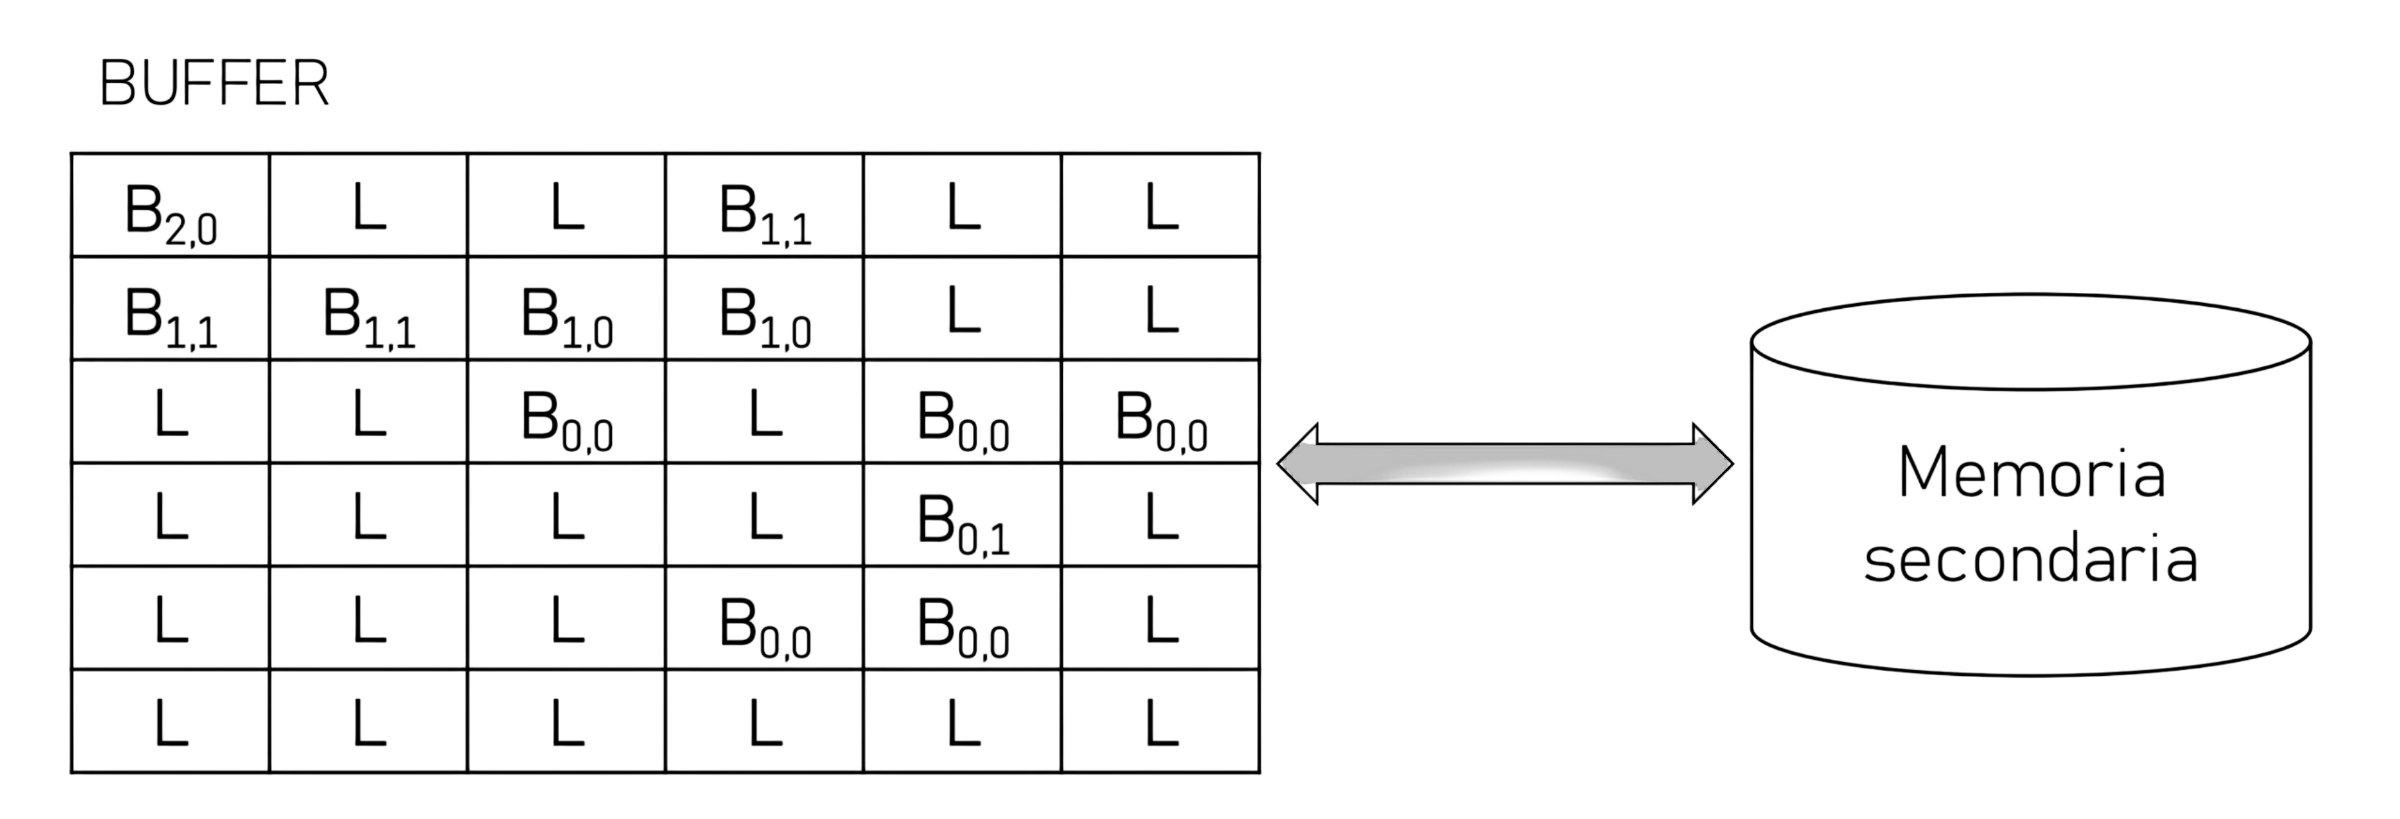
\includegraphics[width=0.6\textwidth]{images/gestione-pagine.png}
\end{figure}

Per ogni pagina del buffer si memorizza:
\begin{itemize}[label=$\triangleright$, itemsep=\smallskipamount]
  \item \textbf{blocco B} (L se libero) indicando il file e il numero di blocco (offset)
  \item \textbf{variabili di stato} ($\mathrm{B_{i,j}}$):
  \begin{itemize}[label=$\circ$, itemsep=\smallskipamount]
    \item \textbf{contatore} $\mathbf{i}$: indica il numero di transazioni
    \item \textbf{bit di stato} $\mathbf{j}$: indica se la pagina è stata modificata (1) o no (0)
  \end{itemize}
\end{itemize}

\subsection{Primitive per la gestione del buffer}

\subsubsection{Primitiva \protect\texttt{fix}}
La \textcolor{azzurrino}{primitiva \texttt{fix}} viene utilizzata dalle transazioni per richiedere l'accesso a un blocco e restituisce un puntatore alla pagina contente il blocco richiesto.

Le azioni della primitiva sono:
\begin{itemize}[label=$\triangleright$, itemsep=\medskipamount]
  \item \textbf{ricerca del blocco}:
  \begin{itemize}[label=$\diamond$, itemsep=\medskipamount]
    \item blocco viene trovato
    \begin{itemize}[label=$\Rightarrow$, itemsep=\smallskipamount]
      \item viene restituito un puntatore alla pagina contentente il blocco
    \end{itemize}
    \item blocco non viene trovato:
    \begin{itemize}[label=$\circ$, itemsep=\smallskipamount]
      \item viene scelta una pagina libera
      \begin{itemize}[label=$\Rightarrow$, itemsep=\smallskipamount]
        \item viene salvata in memoria secondaria (primitiva $\verb|flush|$)
        \item viene caricato il blocco in P aggiornando file e numero di blocco
      \end{itemize}
      \item non ci sono pagine libere
      \begin{itemize}[label=$\Rightarrow$, itemsep=\smallskipamount]
        \item viene rubata una pagina a un'altra transazione (primitiva $\verb|flush|$)
        \item viene sospesa la transazione inserendola in una coda di attesa
        \item se si libera una pagina il gestore si comporterà come al punto precedente
      \end{itemize}
    \end{itemize}
  \end{itemize}
\end{itemize}
\medskip
\begin{itemize}[label=$\Rightarrow$]
  \item \textcolor{red}{\textbf{effetto della modifica}}: quando una transizione accede a una pagina per la prima volta il contatore si incrementa
\end{itemize}

\subsubsection{Primitiva \protect\texttt{unfix}}
La \textcolor{azzurrino}{primitiva \texttt{unfix}} viene usata dalle transazioni per indicare che la transazione ha terminato di usare il blocco.

\begin{itemize}[label=$\Rightarrow$]
  \item \textcolor{red}{\textbf{effetto della modifica}}: decremento del contatore $\mathrm{i}$
\end{itemize}

\subsubsection{Primitiva \protect\texttt{setDirty}}
La \textcolor{azzurrino}{primitiva \texttt{setDirty}} viene utilizzata dalle transazioni per indicare al gestore del buffer che il blocco della pagina è stato modificato.

\begin{itemize}[label=$\Rightarrow$]
  \item \textcolor{red}{\textbf{effetto della modifica}}: bit di stato $\mathrm{j}$ passa da 0 a 1
\end{itemize}

\subsubsection{Primitiva \protect\texttt{force}}
La \textcolor{azzurrino}{primitiva \texttt{force}} viene utilizzata per salvare in memoria secondaria in \hl{modo sincrono} il blocco contenuto nella pagina.\\[0.2ex]
Questa primitiva viene usata dal gestore dell'affidabilità.

\begin{itemize}[label=$\Rightarrow$]
  \item \textcolor{red}{\textbf{effetto della modifica}}: viene salvato in memoria secondaria il blocco e il bit di stato $\mathrm{j}$ posto a 0
\end{itemize}

\subsubsection{Primitiva \protect\texttt{flush}}
La \textcolor{azzurrino}{primitiva \texttt{flush}} viene utilizzata per salvare i blocchi in memoria secondaria in \hl{modo asincrono}.\\[0.2ex]
Questa primitiva viene usata dal gestore del buffer.

\begin{itemize}[label=$\Rightarrow$]
  \item \textcolor{red}{\textbf{effetto della modifica}}: viene liberata la pagina "dirty" e il bit di stato $\mathrm{j}$ viene posto a 0
\end{itemize}

\section{Gestore dell'affidabilità}
Il gestore del buffer differisce le operazioni di scrittura e questo potrebbe rappresentare un pericolo.\\[0.2ex]
Il \textcolor{azzurrino}{\textbf{gestore dell'affibilità}} si occupa di garantire:
\begin{itemize}[label=$\triangleright$, itemsep=\smallskipamount]
  \item \textbf{atomicità}: transazioni non devono essere incomplete
  \item \textbf{persistenza}: effetti di ciascuna transazione non conclusa con un commit devono essere mantenuti in modo permanente
\end{itemize}

\begin{figure}[H]
  \centering
  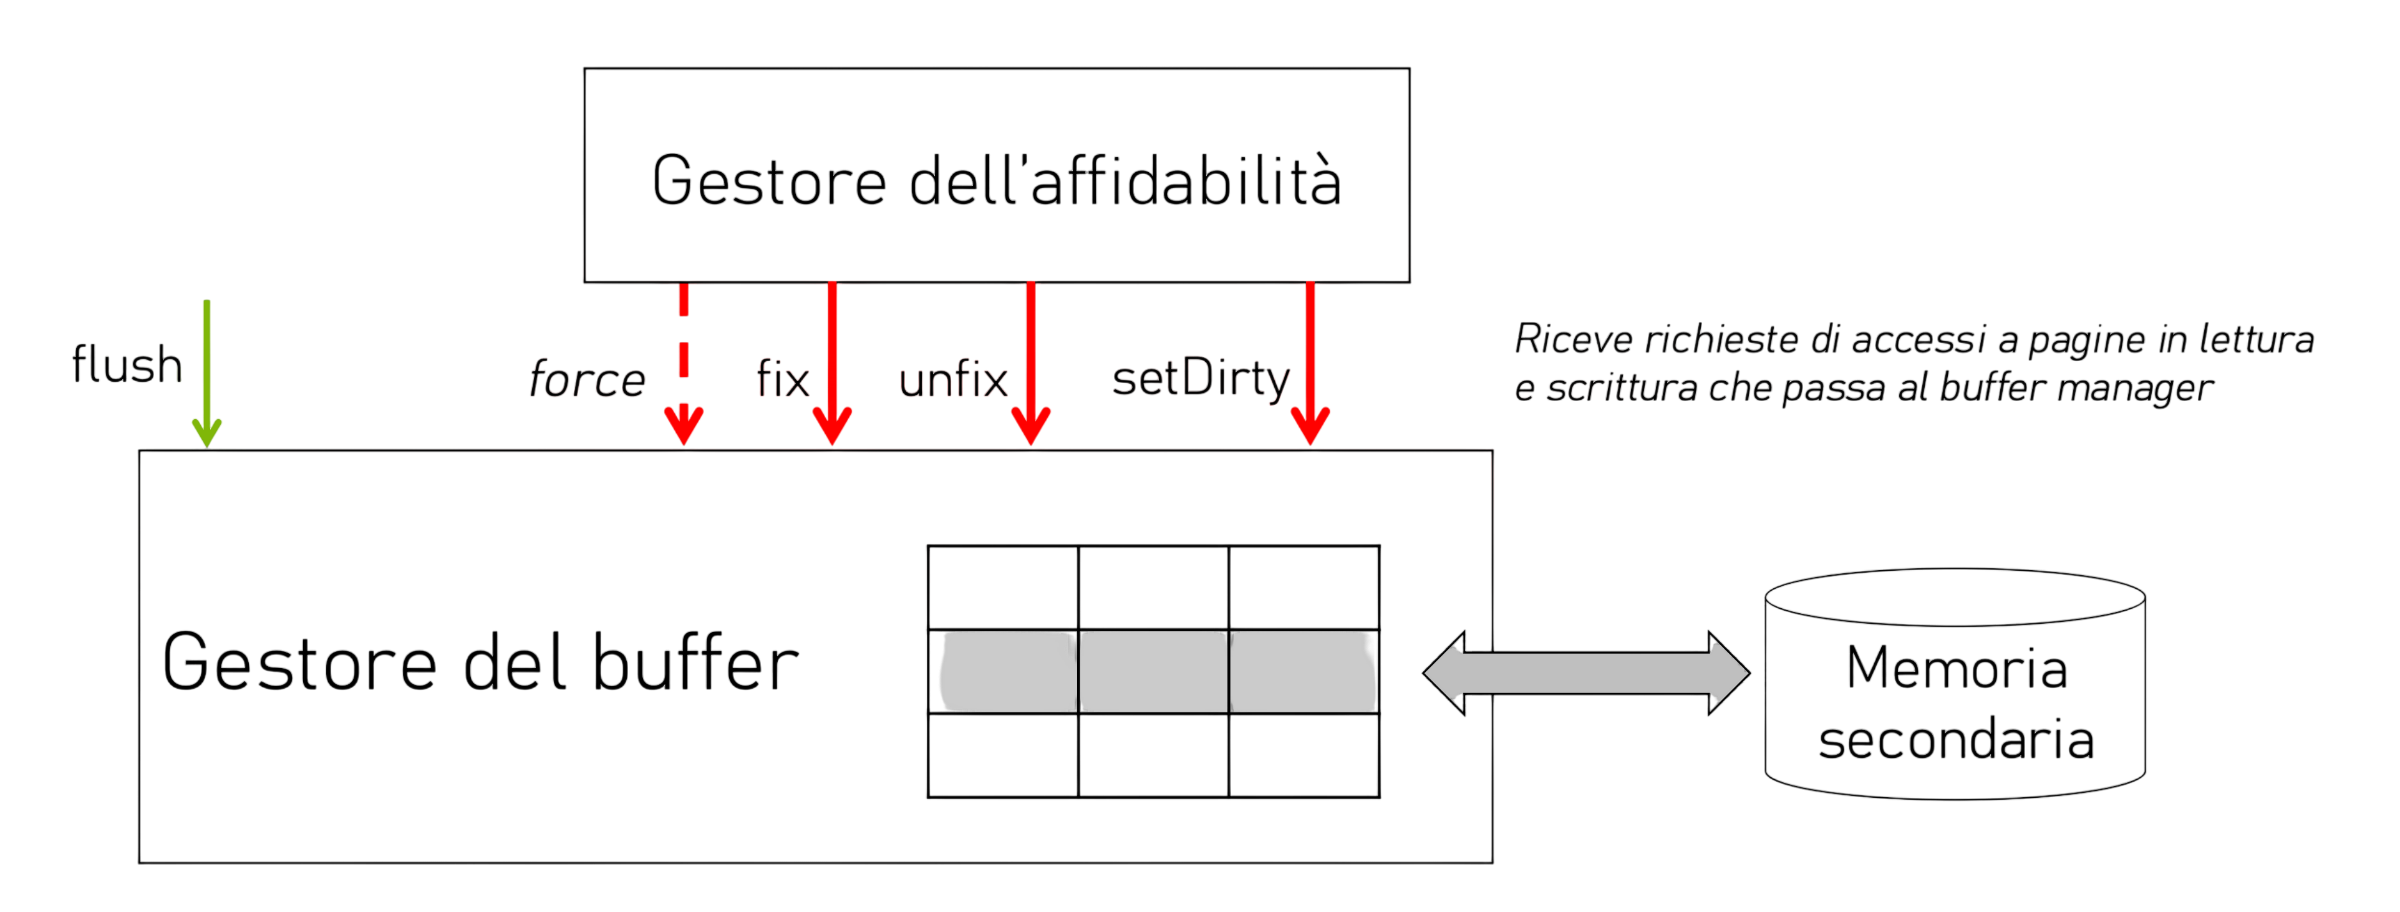
\includegraphics[width=0.6\textwidth]{images/gestore-affidabilità.png}
\end{figure}


\subsection{File di LOG}
Il funzionamento del gestore dell'affidabilità si basa sull'utilizzo del \textbf{file di LOG}.

\definizione{file di LOG}{
  Il \textbf{file di LOG} è un archivio persistente su cui vengono registrate tutte le operazioni eseguite dal DBMS.
}

Per il corretto funzionamento, il gestore dell'affidabilità deve disporre di un dispositivo di \textbf{memoria stabile} (resistente ai guasti).

Il file di LOG viene memorizzato in memoria stabile e al suo interno vengono memorizzati:
\begin{itemize}[label=$\triangleright$, itemsep=\medskipamount]
  \item \textbf{record di transizione}: record che descrivono informazioni sulle transazioni
  \begin{itemize}[label=$\diamond$, itemsep=\smallskipamount]
    \item $\mathbf{B(T)}$: \textcolor{azzurrino}{\textbf{begin}} della transazione
    \item $\mathbf{C(T)}$: \textcolor{azzurrino}{\textbf{commit}} della transazione
    \item $\mathbf{A(T)}$: \textcolor{azzurrino}{\textbf{abort}} della transazione
    \item $\mathbf{I(T,O,AS)}$: \textcolor{azzurrino}{\textbf{insert}} di un oggetto $\mathrm{O}$ da parte di una transazione $\mathrm{T}$ con il suo after state $\mathrm{AS}$ (stato dell'oggetto dopo l'operazione)
    \item $\mathbf{D(T,O,AS)}$: \textcolor{azzurrino}{\textbf{delete}} di un oggetto $\mathrm{O}$ da parte della transizione $\mathrm{T}$ con il suo before state $\mathrm{BS}$ (stato dell'oggetto prima dell'operazione)
    \item $\mathbf{U(T,O,BS,AS)}$: \textcolor{azzurrino}{\textbf{update}} di un oggetto $\mathrm{O}$ da parte della transizione $\mathrm{T}$ con il suo before state $\mathrm{BS}$ e il suo after state $\mathrm{AS}$
  \end{itemize}
  \item \textbf{record di sistema}: record che descrivono informazioni sulle operazioni esaguite dal DBMS
  \begin{itemize}[label=$\circ$, itemsep=\smallskipamount]
    \item $\mathbf{DUMP}$: copia completa e consistente della base di dati.
    \item $\mathbf{CK(T_1, \dots, T_n)}$: indica che all'esecuzione del checkpoint, le transazioni attive erano $\mathrm{T_1, \dots, T_n}$
    \begin{itemize}[itemsep=\smallskipamount]
      \item elenco delle transazioni che non hanno ancora espresso la loro scelta relativamente all'esito finale
      \item operazione svolta periodicamente affinché i dati delle transazioni che hanno eseguito il \texttt{commit} siano registrati in modo permanente
      \item il protocollo di checkpoint prevede i seguenti passi:
      \begin{enumerate}[itemsep=\smallskipamount]
        \item sospensione delle operazioni di \texttt{scrittura}, \texttt{commit} e \texttt{abort} delle transazioni
        \item esecuzione della primitiva \texttt{force} sulle pagine ``dirty'' di transazioni che hanno eseguito il \texttt{commit}
        \item scrittura sincrona (primitiva \texttt{force}) sul file di LOG del record di checkpoint con gli identificatori delle transazioni attive
        \item ripresa delle operazioni di \texttt{scrittura}, \texttt{commit} e \texttt{abort} delle transazioni
      \end{enumerate}
    \end{itemize}
  \end{itemize}
\end{itemize}

I record di transazione salvati nel LOG consentono di eseguire in caso di ripristino le seguenti operazioni:
\begin{itemize}[label=$\triangleright$, itemsep=\smallskipamount]
  \item $\mathbf{UNDO}$: viene usato per disfare un'azione su un oggetto $\mathrm{O}$.
  
  \hl{È sufficiente ricopiare in $\mathrm{O}$ il valore d $\mathrm{BS}$}.
  
  L'\texttt{insert}/\texttt{delete} viene disfatto cancellando/inserendo $\mathrm{O}$
  \item $\mathbf{REDO}$: serve per rifare un'azione su un oggetto $\mathrm{O}$.
  
  \hl{È sufficiente ricopiare in $\mathrm{O}$ il valore $\mathrm{AS}$}.
  
  L'\texttt{insert}/\texttt{delete} viene rifatto inserendo/cancellando $\mathrm{O}$
\end{itemize}

\medskip
Gli inserimenti controllano sempre l’esistenza di $\mathrm{O}$ prima di eseguire l'operazione.\\[0.2ex]
Per queste operazioni vale la \textbf{proprietà di idempotenza}.

\definizione{proprietà di idempotenza}{
  \[
    \begin{aligned}
      \mathrm{UNDO(UNDO(A))} &= \mathrm{UNDO(A)}\\
      \mathrm{REDO(REDO(A))} &= \mathrm{REDO(A)}
    \end{aligned}
  \]
}

\subsection{Regole di scrittura sul file di LOG}
Il gestore dell'affidabilità deve rispettare le seguenti regole di scrittura sul file di LOG:
\begin{itemize}[label=$\Rightarrow$, itemsep=\smallskipamount]
  \item \textbf{regola Write Ahead Logging}: record di LOG devono essere scritti sul LOG precedente all'esecuzione delle corrispondenti operazioni sulla base di dati (garantisce la possibilità di fare sempre \texttt{UNDO})
  \item \textbf{regola di commit-precedenza}: record di LOG devono essere scritti sul LOG prima dell'esecuzione del \texttt{commit} della transazione (garantisce la possibilità di fare sempre \texttt{REDO})
\end{itemize}

Queste regole consentono di salvare i blocchi delle pagine “dirty” in modo totalmente asincrono rispetto al commit delle transazioni.

\subsection{Guasti}
Una transazione $\mathrm{T}$ sceglie in modo atomico l'esito di $\verb|commit|$ nel momento in cui scrive nel file di LOG in modo sincrono (primitiva $\verb|force|$) il suo record di $\verb|commit| \ \mathrm{C(T)}$. 

\begin{itemize}[label=$\Rightarrow$, itemsep=\smallskipamount]
  \item se avviene un guasto prima della scrittura del record di $\verb|commit|$ $\rightarrow$ $\mathbf{UNDO}$
  \item se avviene un guasto dopo la scrittura del record di $\verb|commit|$ $\rightarrow$ $\mathbf{REDO}$
\end{itemize}

Esistono due tipologie di guasto:
\begin{itemize}[label=$\triangleright$, itemsep=\medskipamount]
  \item \textbf{guasto di sistema}: perdita del contenuto della memoria centrale.
  
  Viene risolto con la tecnica della \textcolor{azzurrino}{\textbf{ripresa a caldo}}:
  \begin{enumerate}[itemsep=\smallskipamount]
    \item accede al file di LOG e si ripercorre all’indietro il LOG fino al più recente record di checkpoint
    \item si inizializza:
    \begin{itemize}[label=$\diamond$, itemsep=\smallskipamount]
      \item insieme $\mathrm{UNDO}$ con tutte le transazioni da disfare (presenti nel checkpoint)
      \item insieme $\mathrm{REDO}$ con tutte le transazioni da rifare ($\emptyset$)
    \end{itemize}
    \item si ripercorre in avanti il LOG
    \begin{itemize}[label=$\circ$, itemsep=\smallskipamount]
      \item per ogni record $\mathrm{B(T)}$ incontrato si aggiunge $\mathrm{T}$ all’insieme $\mathrm{UNDO}$
      \item per ogni record $\mathrm{C(T)}$ incontrato si sposta $\mathrm{T}$ dall’insieme $\mathrm{UNDO}$ all’insieme $\mathrm{REDO}$
    \end{itemize}
    \item si ripercorre all'indietro il LOG disfacendo le operazioni eseguite dalle transazioni $\mathrm{UNDO}$ risalendo fino alla prima azione della transazione più vecchia
    \item si ripercorre in avanti il LOG per rifare le operazioni eseguite dalle transazioni $\mathrm{REDO}$
  \end{enumerate}
  \item \textbf{guasto di dispositivo}: perdita di parte o tutto il contenuto della base di dati in memoria secondaria.
  
  Viene risolto con la tecninca della \textcolor{azzurrino}{\textbf{ripresa a freddo}}:
  \begin{enumerate}[itemsep=\smallskipamount]
    \item si accede al $\mathrm{DUMP}$ della base di dati e si ricopia selettivamente la parte deteriorata della base di dati
    \item si accede al LOG risalendo al record di $\mathrm{DUMP}$
    \item si ripercorre in avanti il LOG rieseguendo tutte le operazioni relative alla parte deteriorata comprese le azioni di $\verb|commit|$ e $\verb|abort|$
    \item si applica una ripresa a caldo
  \end{enumerate}
\end{itemize}

\esercizio{file di LOG}{
  Consideriamo il seguente file di LOG:
  \[
    \begin{aligned}
      & \mathrm{B(T_1), B(T_2), U(T_2, O_1, B_1, A_1), I(T_1, O_2, A_2), B(T_3), C(T_1), B(T_4),} \\
      & \mathrm{U(T_3, O_2, B_3, A_3), U(T_4, O_3, B_4, A_4), CK(T_2, T_3, T_4), C(T_4), B(T_5),} \\
      & \mathrm{U(T_3, O_3, B_5, A_5), U(T_5, O_4, B_6, A_6), D(T_3, O_5, B_7), A(T_3), C(T_5),} \\
      & \mathrm{I(T_2, O_6, A_8)} \text{ \textbf{guasto}}
    \end{aligned}
  \] 

  \textcolor{red}{\textbf{Che passi svolge la ripresa a caldo?}}
  \begin{enumerate}
    \item risale il LOG fino all'ultimo record di checkpoint $\mathrm{CK(T_2,T_3,T_4)}$
    \smallskip
    \item inizializza $\mathrm{UNDO}$ e $\mathrm{REDO}$
    \begin{itemize}[label=$\triangleright$]
      \item $\mathrm{UNDO = \{T_2, T_3, T_4\}}$ (inizializzato con le transazioni del checkpoint)
      \smallskip
      \item $\mathrm{REDO = \emptyset}$ 
    \end{itemize}
    \smallskip
    \item ripercorre in avanti il LOG dal CheckPoint fino al guasto e si aggiungono o si spostano le transazioni tra $\mathrm{UNDO}$ e $\mathrm{REDO}$
    \begin{itemize}[label=$\triangleright$]
      \item $\mathrm{UNDO = \{T_2, T_3, \cancel{T_4}, \cancel{T_5}\}}$ (inizializzato con le transazioni del checkpoint)
      \smallskip
      \item $\mathrm{REDO = \{T_4, T_5\}}$ 
    \end{itemize}
    \smallskip
    \item ripercorre all’indietro il LOG disfacendo le operazioni eseguite dalle transazioni $\mathrm{UNDO}$ risalendo fino alla prima azione della transazione più vecchia
    \[
      \begin{aligned}
        &\mathrm{DELETE(O_6) \quad (\text{disfare} \ \texttt{insert})}\\
        &\mathrm{O_5 := B_7  \quad (\text{disfare} \ \texttt{delete})}\\
        &\mathrm{O_3 := B_5 \quad (\text{disfare} \ \texttt{update})}\\
        &O_2 := B_3 \ \quad (\text{disfare} \ \texttt{update})\\
        &\mathrm{O_1 := B_1 \quad (\text{disfare} \ \texttt{update})}\\
      \end{aligned}
    \]
    \smallskip
    \item  ripercorre in avanti il LOG per rifare le operazioni eseguite dalle transazioni $\mathrm{REDO}$
    \[
      \begin{aligned}
        &\mathrm{O_3 := A_4  \quad (\text{rifare} \ \texttt{update})}\\
        &\mathrm{O_4 := A_6 \quad (\text{rifare} \ \texttt{update})}\\
      \end{aligned}
    \]
  \end{enumerate}
}

\esercizio{file di LOG}{
  Consideriamo il seguente file di LOG:
  \[
    \begin{aligned}
      &\mathrm{B(T_1), B(T_2), B(T_3), I(T_1, O_1, A_1), D(T_2, O_2, B_2), B(T_4),} \\
      &\mathrm{U(T_4, O_3, B_3, A_3), U(T_1, O_4, B_4, A_4), C(T_2), CK(T_1, T_3, T_4), B(T_5), B(T_6),} \\
      &\mathrm{U(T_5, O_5, B_5, A_5), A(T_3), CK(T_1, T_4, T_5, T_6), B(T_7), C(T_4),} \\
      &\mathrm{U(T_7, O_6, B_6, A_6), U(T_6, O_3, B_7, A_7), B(T_8), A(T_7)} \text{ \textbf{guasto}}
    \end{aligned}
  \]

  \textcolor{red}{\textbf{Che passi svolge la ripresa a caldo?}}
  \begin{enumerate}
    \item risale il LOG fino all'ultimo record di checkpoint $\mathrm{CK(T_1,T_4,T_5,T_6)}$
    \smallskip
    \item inizializza $\mathrm{UNDO}$ e $\mathrm{REDO}$
    \begin{itemize}[label=$\triangleright$]
      \item $\mathrm{UNDO = \{T_1, T_4, T_5, T_6\}}$ (inizializzato con le transazioni del checkpoint)
      \smallskip
      \item $\mathrm{REDO = \emptyset}$ 
    \end{itemize}
    \smallskip
    \item ripercorre in avanti il LOG dal checkpoint fino al guasto e si aggiungono o si spostano le transazioni tra $\mathrm{UNDO}$ e $\mathrm{REDO}$
    \begin{itemize}[label=$\triangleright$, itemsep=\smallskipamount]
      \item $\mathrm{UNDO = \{T_1, \cancel{T_4}, T_5, t_6, t_7, t_8\}}$ (inizializzato con le transazioni del checkpoint)
      \item $\mathrm{REDO = \{T_4\}}$ 
    \end{itemize}
    \smallskip
    \item ripercorre all’indietro il LOG disfacendo le operazioni eseguite dalle transazioni $\mathrm{UNDO}$ risalendo fino alla prima azione della transazione più vecchia
    \[
      \begin{aligned}
        &\mathrm{O_3 := B_7  \quad (\text{disfare} \ \texttt{update})}\\
        &\mathrm{O_6 := B_6 \quad (\text{disfare} \ \texttt{update})}\\
        &\mathrm{O_5 := B_5 \quad (\text{disfare} \ \texttt{update})}\\
        &\mathrm{O_4 := B_4  \quad (\text{disfare} \ \texttt{update})}\\
        &\mathrm{DELETE(O_1) \quad (\text{disfare} \ \texttt{insert})}\\
      \end{aligned}
    \]
    \smallskip
    \item  ripercorre in avanti il LOG per rifare le operazioni eseguite dalle transazioni $\mathrm{REDO}$
    \[
      \begin{aligned}
        &\mathrm{O_3 := A_3  \quad (\text{rifare} \ \texttt{update})}\\
      \end{aligned}
    \]
  \end{enumerate}
}

\section{Gestore dei metodi di accesso}
Il \textcolor{azzurrino}{\textbf{gestore dei metodi di accesso}} esegue il piano di esecuzione prodotto dall'ottimizzatore e produce sequenze di richieste di accessi ai blocchi della base di dati presenti in memoria secondaria.\\[0.2ex]
Le richieste vengono inviate al gestore del buffer che si occupa di caricare i blocchi necessari in pagine di memoria centrale.

\begin{figure}[H]
  \centering
  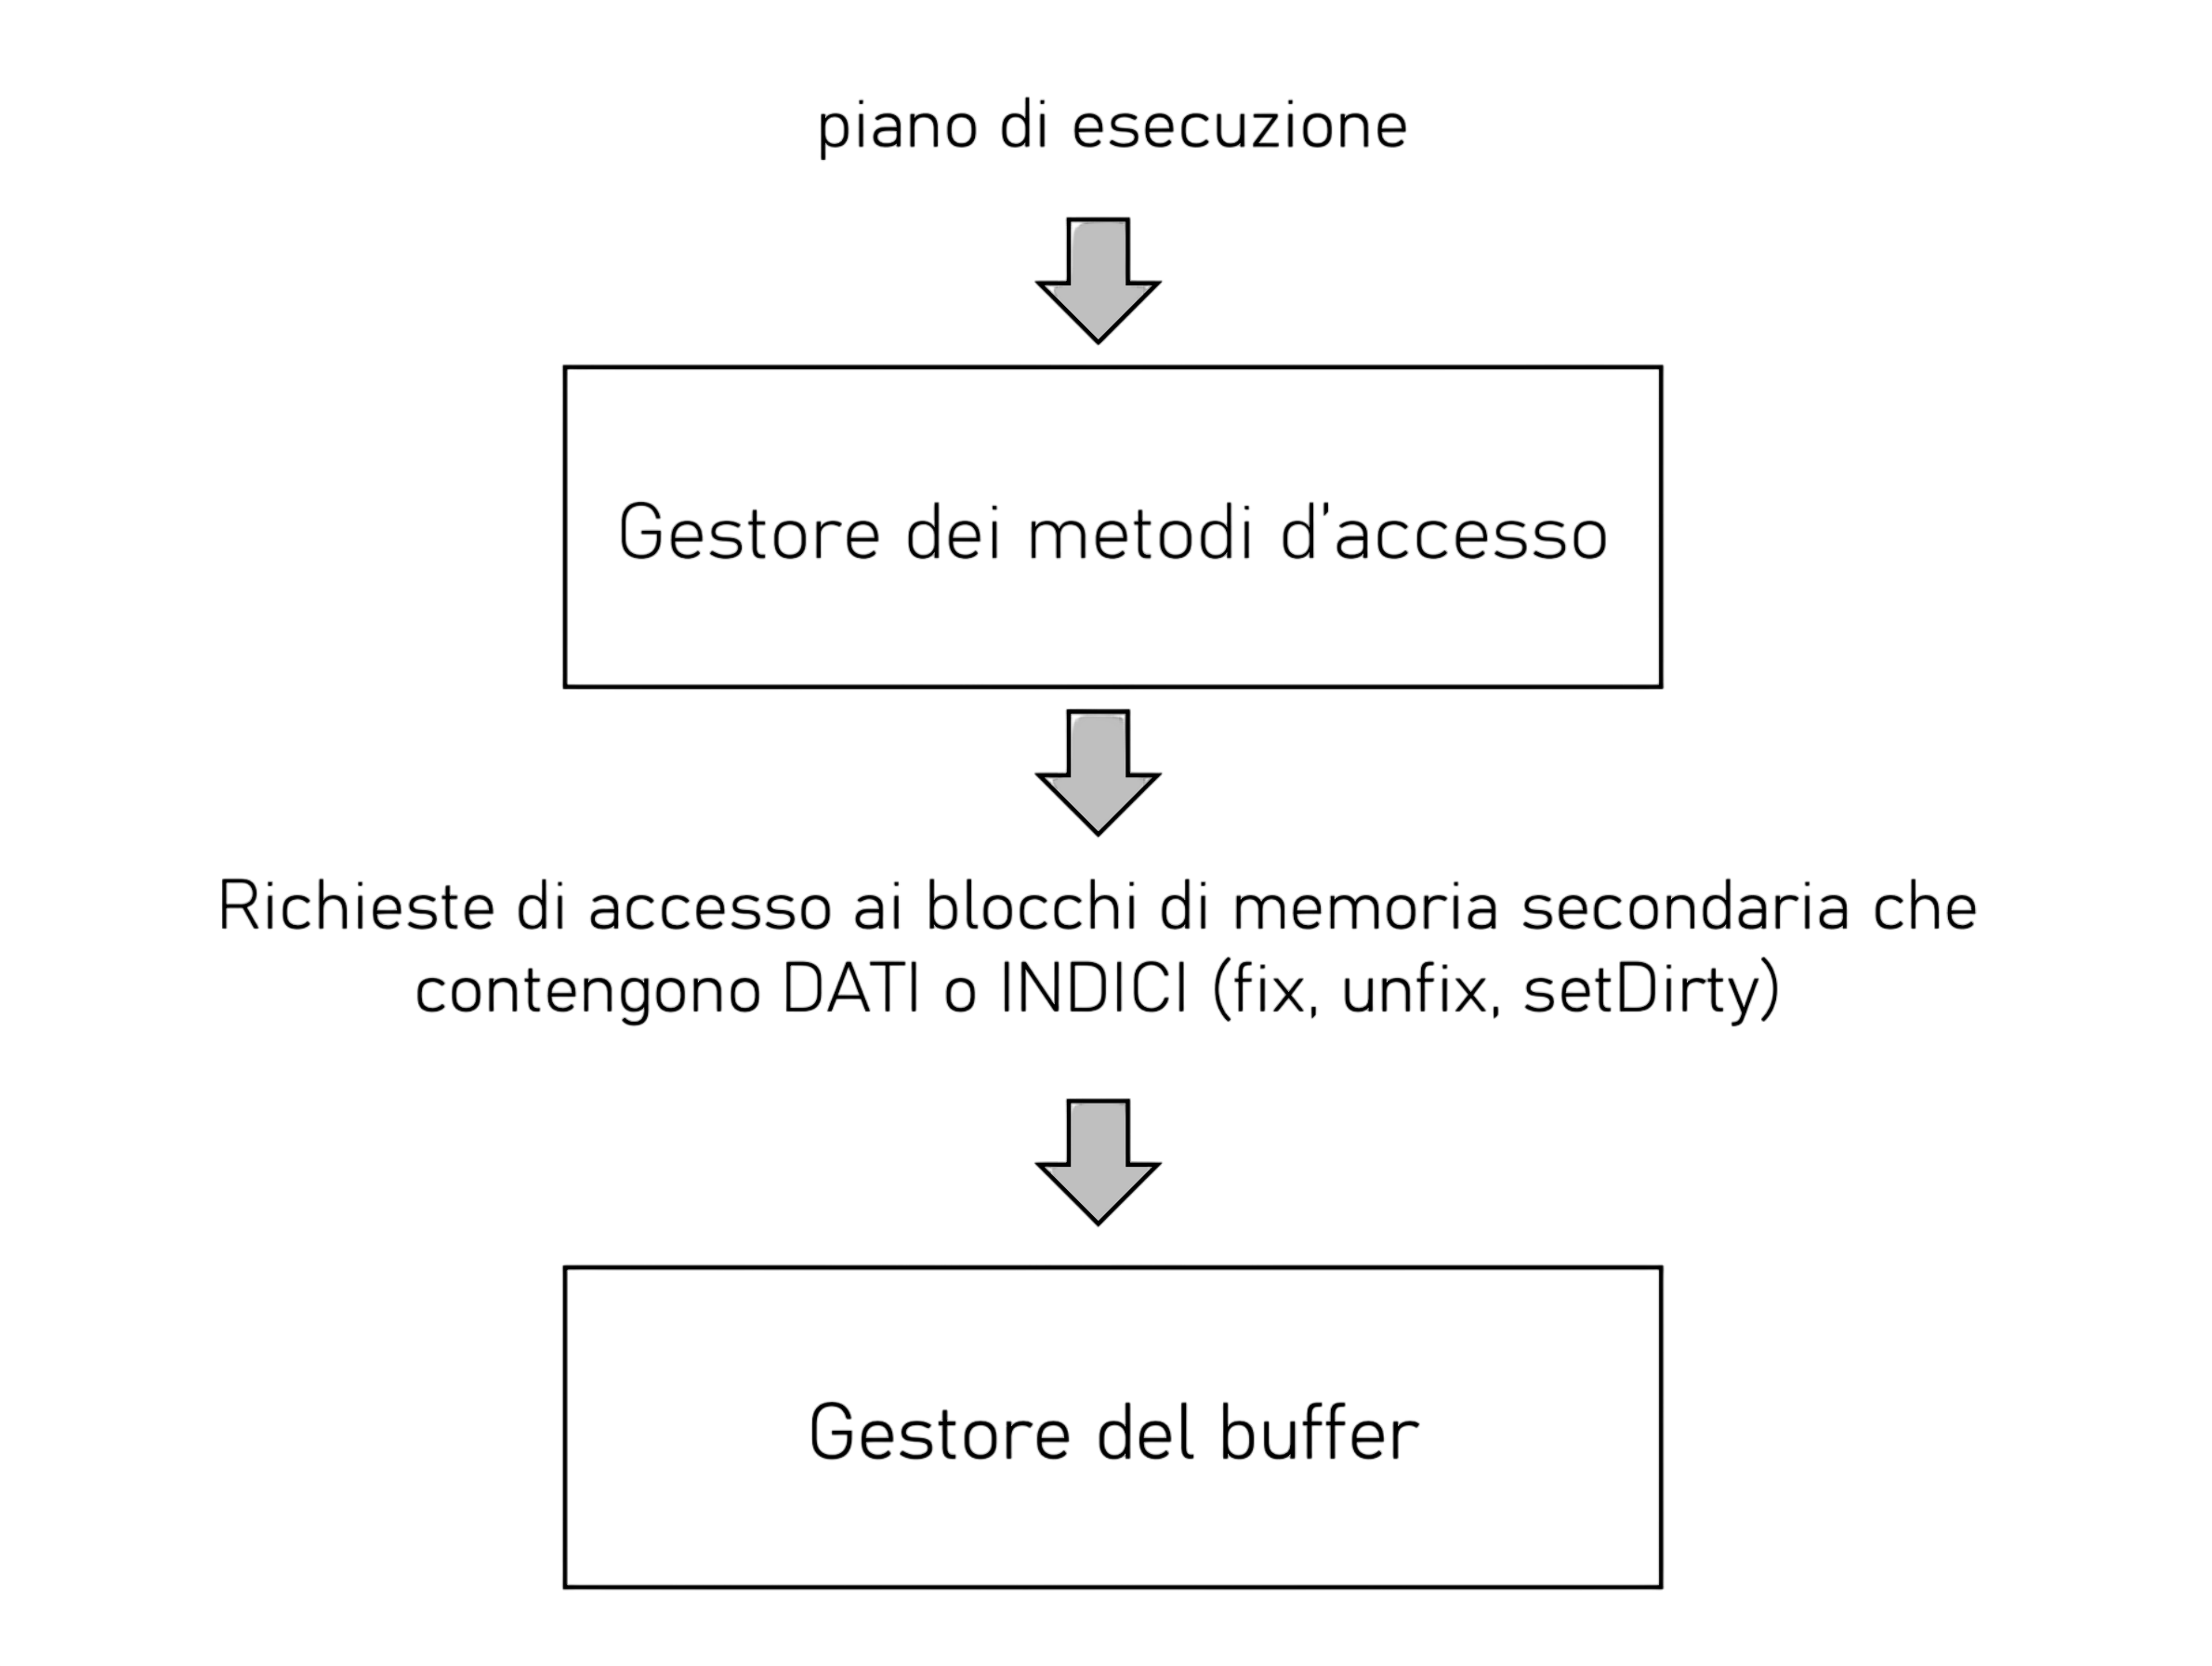
\includegraphics[width=0.6\textwidth]{images/gestore-accesso.png}
  \caption{gestore dei meotodi di accesso}
\end{figure}

\subsection{Metodi di accesso}
I metodi di accesso sono \textbf{moduli software} (es. scansione sequenziale, accesso via indice, ordinamento, varie implementazioni del join) che implementano gli algoritmi di accesso e manipolazione dei dati organizzati in specifiche strutture fisiche.

Ogni metodo di accesso conosce:
\begin{itemize}[label=$\diamond$, itemsep=\smallskipamount]
  \item \textbf{organizzazione in tuple} (o dei record di indice) nei blocchi dati (indice) salvati in memoria secondaria
  \item \textbf{organizzazione fisica interna delle pagine} sia quando contengono dati, sia quando contengono strutture fisiche di accesso (indici)
\end{itemize}

\subsection{Organizzazione di una pagina}
All'interno di una pagina sono presenti:
\begin{itemize}[label=$\triangleright$, itemsep=\smallskipamount]
  \item \textbf{informazioni utili}: dati veri e propri (tuple della tabella)
  \item \textbf{informazioni di controllo}: consentono di accedere alle informazioni utili (dizionario, bit di parità, altre informazioni del file system o della specifica struttura fisica)
\end{itemize}

\begin{figure}[H]
  \centering
  \includegraphics[width=0.6\textwidth]{images/organizzazione-pagina.png}
  \caption{organizzazione di una pagina}
\end{figure}

\begin{itemize}[label=$\Rightarrow$, itemsep=\smallskipamount]
  \item \textcolor{red}{\textbf{blocco header/trailer}}: contengono informazioni di controllo utilizzate dal file system
  \item \textcolor{violet}{\textbf{pagina header/trailer}}: contengono le informazioni di controllo relative alla specifica struttura fisica
  \item \textcolor{orange}{\textbf{dizionario di pagina}}: contiene i puntatori a ciascun dato utile elementare contenuto nella pagina
  \item \textcolor{green}{\textbf{bit di parità}}: verifica che l'informazione contenuta nella pagina sia valida
  \item \textcolor{blue}{\textbf{parte utile}}: contiene i dati
\end{itemize}

\vario{Nota}{
  Dizionari di pagina e parte utile crescono come stack contrapposti lasciando libera la parte centrale in uno spazio contiguo.
}

In caso di \textbf{tuple di lunghezza fissa}, il dizionario non è necessario: si memorizza la dimensione delle tuple e l'offset del punto iniziale.

\smallskip
In caso di \textbf{tuple di lunghezza variabile}, il dizionario memorizza l'offset di ogni tupla presente nel blocco e di ogni attributo di ogni tupla.

Molti gestori delle pagine non consentono la separazione di una tupla su più pagine:
\begin{equation*}
  \text{dimensione massima tupla} = \text{dimensione massima area disponibile su un blocco}
\end{equation*}

Alcuni gestori delle pagine consentono di distribuire una tupla su più pagine, altrimenti va gestito il caso di tuple memorizzate su più pagine.

\subsection{Operazioni sulle pagine}
Le principali operazioni che si possono eseguire sulle pagine sono:
\begin{itemize}[label=$\triangleright$, itemsep=\smallskipamount]
  \item \textbf{inserimento/aggiornamento di una tupla}:
  \begin{itemize}[label=$\diamond$, itemsep=\smallskipamount]
    \item esiste spazio contiguo sufficiente: \texttt{inserimento}
    \item non esiste spazio contiguo sufficiente, ma spazio sufficiente: \texttt{riorganizzazione dello spazio + inserimento}
    \item non esiste spazio sufficiente: \texttt{interazione con il file system per allocare nuovi blocchi per il file}
  \end{itemize}
  \item \textbf{cancellazione contenuto della pagina}
  \item \textbf{accesso a una tupla}: avviene tramite il valore della chiave o l'offset nel dizionario
  \item \textbf{accesso a un attributo di una tupla}: identificato in base all’offset e alla lunghezza del campo dopo aver identificato la tupla tramite la chiave o il suo offset 
\end{itemize}


\subsection{Strutture primarie per l'organizzazione dei file}
La struttura prmaria di un file stabilisce il criterio di disposizione delle tuple all'interno del file presente in memoria di massa:
\begin{itemize}[label=$\triangleright$, itemsep=\smallskipamount]
  \item \textbf{sequenziale}: colloca le tuple in maniera consecutiva sulla base di un criterio specifico (es. ordine di inserimento)
  \item \textbf{ad accesso calcolato}: colloca le tuple in posizioni determinate sulla base dell'esecuzione di un algoritmo di hash
  \item \textbf{ad albero}: utilizzate come strutture secondarie (indici)
\end{itemize}

\begin{figure}[H]
  \centering
  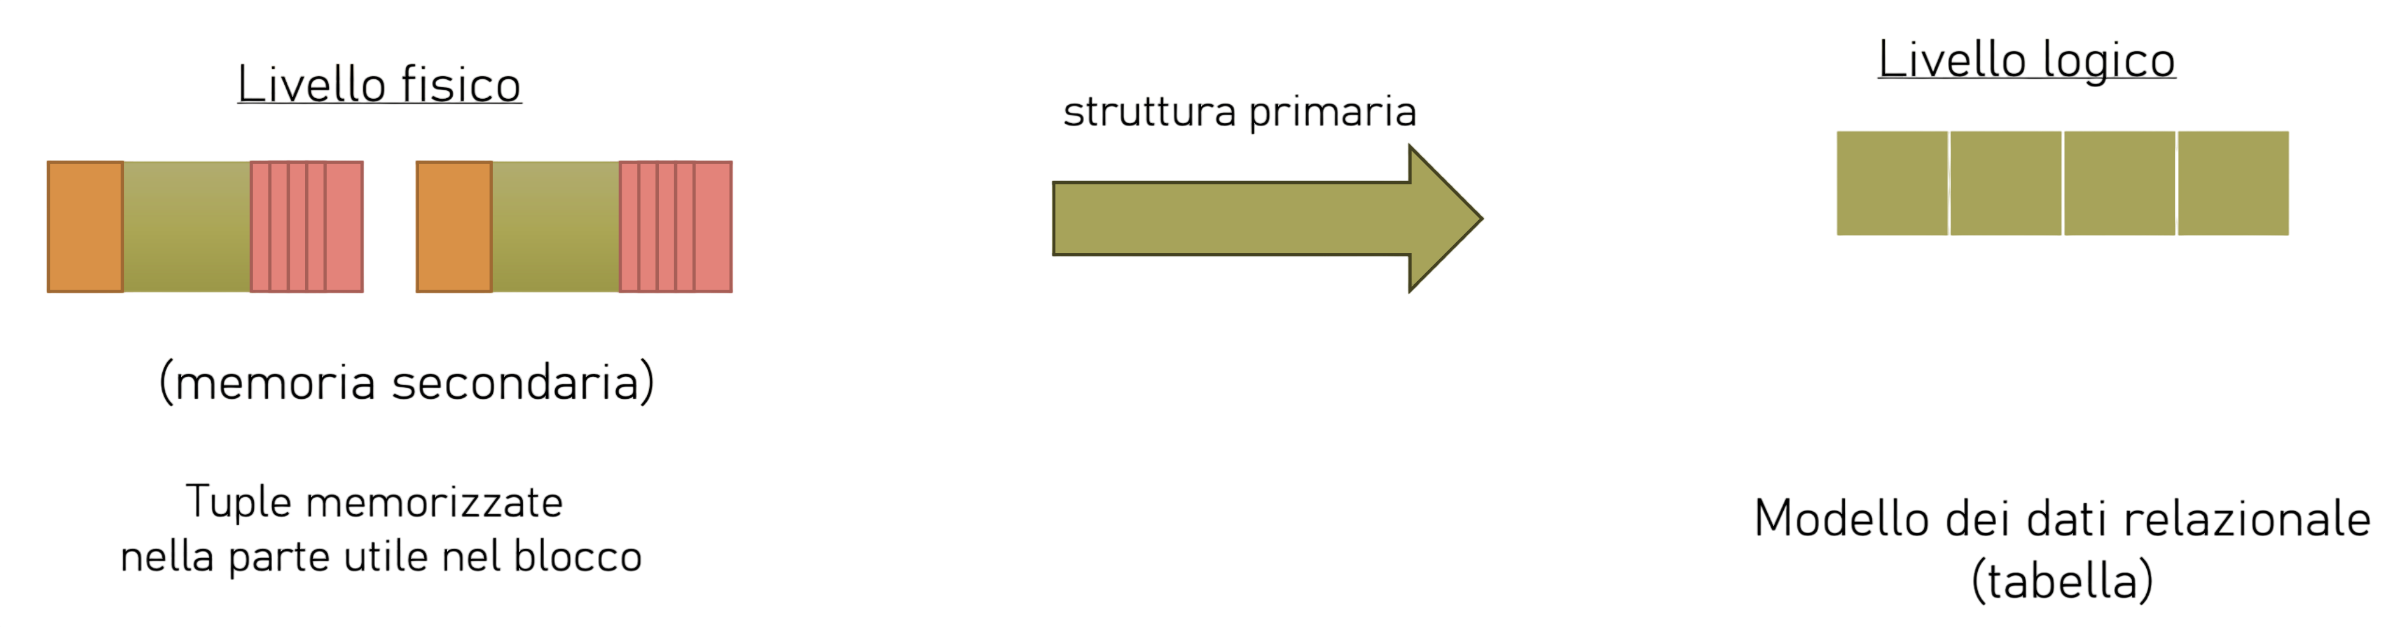
\includegraphics[width=0.7\textwidth]{images/strutture-primarie.png}
  \caption{strutture primarie per l'organizzazione dei file}
\end{figure}

\subsubsection{Struttura sequenziale}
Un file è costituito da blocchi "logicamente" consecutivi e le tuple vengono inserite nei blocchi rispettando una sequenza.

\paragraph{Struttura sequenziale disordinata}
Le tuple sono disposte in base al loro ordine di inserimento, senza alcun criterio specifico.\\[0.2ex]
Questa è la struttura più semplice e più diffusa.

\begin{itemize}[label=$\Rightarrow$, itemsep=\smallskipamount]
  \item \textbf{inserimento}:
  \begin{itemize}[label=$\diamond$, itemsep=\smallskipamount]
    \item operazione molto efficiente
    \item sufficiente mantenere un riferimento all'ultimo blocco
    \item richiede solo un accesso in memoria secondaria
    \item maggiore costo in caso di verifica dei vincoli di integrità
  \end{itemize}
  \item \textbf{ricerca}
  \begin{itemize}[label=$\diamond$, itemsep=\smallskipamount]
    \item operazione non efficiente
    \item richiede ogni volta una scansione sequenziale che consideri tutti i record, con un costo lineare nel numero di blocchi
    \item ricerca può essere fatta usando strutture secondarie (indici)
  \end{itemize}
  \item \textbf{eliminazione}
  \begin{itemize}[label=$\diamond$, itemsep=\smallskipamount]
    \item  facile una volta individuate le tuple coinvolte
    \item si marcano le tuple come "cancellate" senza riorganizzazione locale
  \end{itemize}
  \item \textbf{modifica}
  \begin{itemize}[label=$\diamond$, itemsep=\smallskipamount]
    \item  facile una volta individuate le tuple coinvolte
    \item si procede in loco se possibile, cioè quando non c’è stata nessuna modifica alla dimensione della tupla
    \item si procede con una cancellazione e un inserimento in fondo al file
  \end{itemize}
\end{itemize}

Eliminazioni e modifiche possono portare a un uso non ottimale dello spazio, siccome, si devono effettuare riorganizzazioni periodiche.

\paragraph{Struttura sequenziale ad array}
Le tuple sono disposte come in un array e la loro posizione dipende dal valore assunto in ciascuna tupla da un campo detto \textbf{indice}.\\[0.2ex]
Questa struttura è utilizzabile soltanto quando le tuple di una tabella
hanno una dimensione fissa, infatti non è quasi masi usata nei DBMS reali perchè difficilmente sono soddisfatte le condizioni per la sua applicazione.

Ad ogni file viene assegnato un numero $\mathbf{n}$ di blocchi contigui e ciascun blocco è dotato di un numero $\mathrm{m}$ di posizioni disponibili per le tuple (array bidimensionale $\mathrm{n \times m}$).\\[0.2ex]
Ogni tupla è dotata di un valore numerico $\mathrm{i}$ che rappresenta l'indice della tupla in i-esima posizione nell'array.

\begin{itemize}[label=$\Rightarrow$, itemsep=\smallskipamount]
  \item \textbf{inserimento}
  \begin{itemize}[itemsep=\smallskipamount]
    \item iniziale: l’indice $\mathbf{i}$ viene ottenuto incrementando un contatore
    \item successivo: in una posizione libera oppure alla fine del file
  \end{itemize}
  \item \textbf{cancellazione}: creano delle posizioni libere
\end{itemize}

\paragraph{Struttura sequenziale ordinata}
È un file sequenziale dove le tuple sono ordinate secondo una chiave di ordinamento (diversa dalla chiave primaria).\\[0.2ex]
Questa struttura rende efficienti le operazioni che hanno bisogno
dell'ordinamento utilizzato, ad esempio:
\begin{itemize}[label=$\circ$, itemsep=\smallskipamount]
  \item elenco ordinato
  \item range query
  \item operazioni aggregate
\end{itemize}

In caso di aggiornamento è necessario mantenere l'ordinamento, quindi servono periodiche riorganizzazioni.

\begin{itemize}[label=$\Rightarrow$, itemsep=\smallskipamount]
  \item \textbf{inserimento}
  \begin{enumerate}[itemsep=\smallskipamount]
    \item individuare il blocco B che contiene la tupla che precede, nell’ordine della chiave, la tupla da inserire
    \item se B contiene spazio sufficiente per la nuova tupla allora si inserisce la tupla in B
    \item altrimenti si aggiunge un nuovo blocco (overflow page) alla struttura e si inserisce la tupla nel nuovo blocco e si aggiusta la catena di puntatori
  \end{enumerate}
  \item \textbf{scansione sequenziale ordinata secondo la chiave}:  è sufficiente seguire i puntatori
  \item \textbf{cancellazione di una tupla}
  \begin{enumerate}[itemsep=\smallskipamount]
    \item individuare il blocco B che contiene la tupla da cancellare
    \item cancellare la tupla da B
    \item aggiustare la catena di puntatori
  \end{enumerate}
  \item \textbf{riorganizzazione}: si assegnano le tuple ai blocchi in base a opportuni coefficienti di riempimento, riaggiustando i puntatori
\end{itemize}

\esempio{struttura sequenziale}{
  Il seguente esempio mostra una struttura sequenziale ordinata secondo la chiave $\texttt{Filiale}$.
  
  \begin{figure}[H]
    \centering
    \includegraphics[width=0.7\textwidth]{images/esempio-struttura-sequenziale.png}
  \end{figure}
}

\paragraph{Indice}
Per aumentare le prestazioni degli accessi alle tuple memorizzate nelle strutture fisiche (file sequenziale), si introducono strutture ausiliarie dette strutture di accesso
ai dati (indici).\\[0.2ex]
Queste strutture velocizzano l'accesso casuale via chiave di ricerca, cioè un insieme di attributi utilizzati nell'indice della ricerca.

Ci sono due tipi di indici su file sequenziali:
\begin{itemize}[label=$\triangleright$, itemsep=\medskipamount]
  \item \textbf{indice primario}: la chiave di ordinamento del file sequenziale coincide con la chiave di ricerca dell’indice.
  
  Ogni record dell’indice primario contiene una coppia $\mathbf{\langle v_i, p_i\rangle}$, dove:
  \begin{itemize}
    \item $\mathrm{v_i}$: valore della chiave di ricerca
    \item $\mathrm{p_i}$: puntatore al primo record nel file sequenziale con chiave $\mathrm{v_i}$
  \end{itemize}

  \smallskip
  Esistono due varianti dell'indice primario:
  \begin{itemize}[itemsep=\smallskipamount]
    \item \textbf{indice denso}: per ogni occorrenza della chiave presente nel file esiste un corrispondente record nell'indice
    \item \textbf{indice sparso}: solo per alcune occorrenze della chiave presenti nel file esiste un corrispondente record nell’indice, tipicamente una per blocco
  \end{itemize}

  \smallskip
  Le operazioni che si possono eseguire su un indice primario sono:
  \begin{itemize}[label=$\diamond$, itemsep=\medskipamount]
    \item \textbf{ricerca di una tupla con chiave di ricerca K}
    \begin{itemize}[label=$\circ$, itemsep=\smallskipamount]
      \item se l'indice è denso $\mathrm{K} \rightarrow$ è presente nell'indice
      \begin{enumerate}[itemsep=\smallskipamount]
        \item scansione sequenziale dell'indice per trovare il record $\mathrm{(K, p_k)}$
        \item accesso al file attraverso il puntatore $\mathrm{p_k}$
      \end{enumerate}

      $\Rightarrow$ \hl{\textbf{costo}: 1 accesso indice + 1 accesso blocco dati}

      \esempio{ricerca con indice primario denso}{
        Un esempio di ricerca con indice primario denso è il seguente:
        \begin{figure}[H]
          \centering
          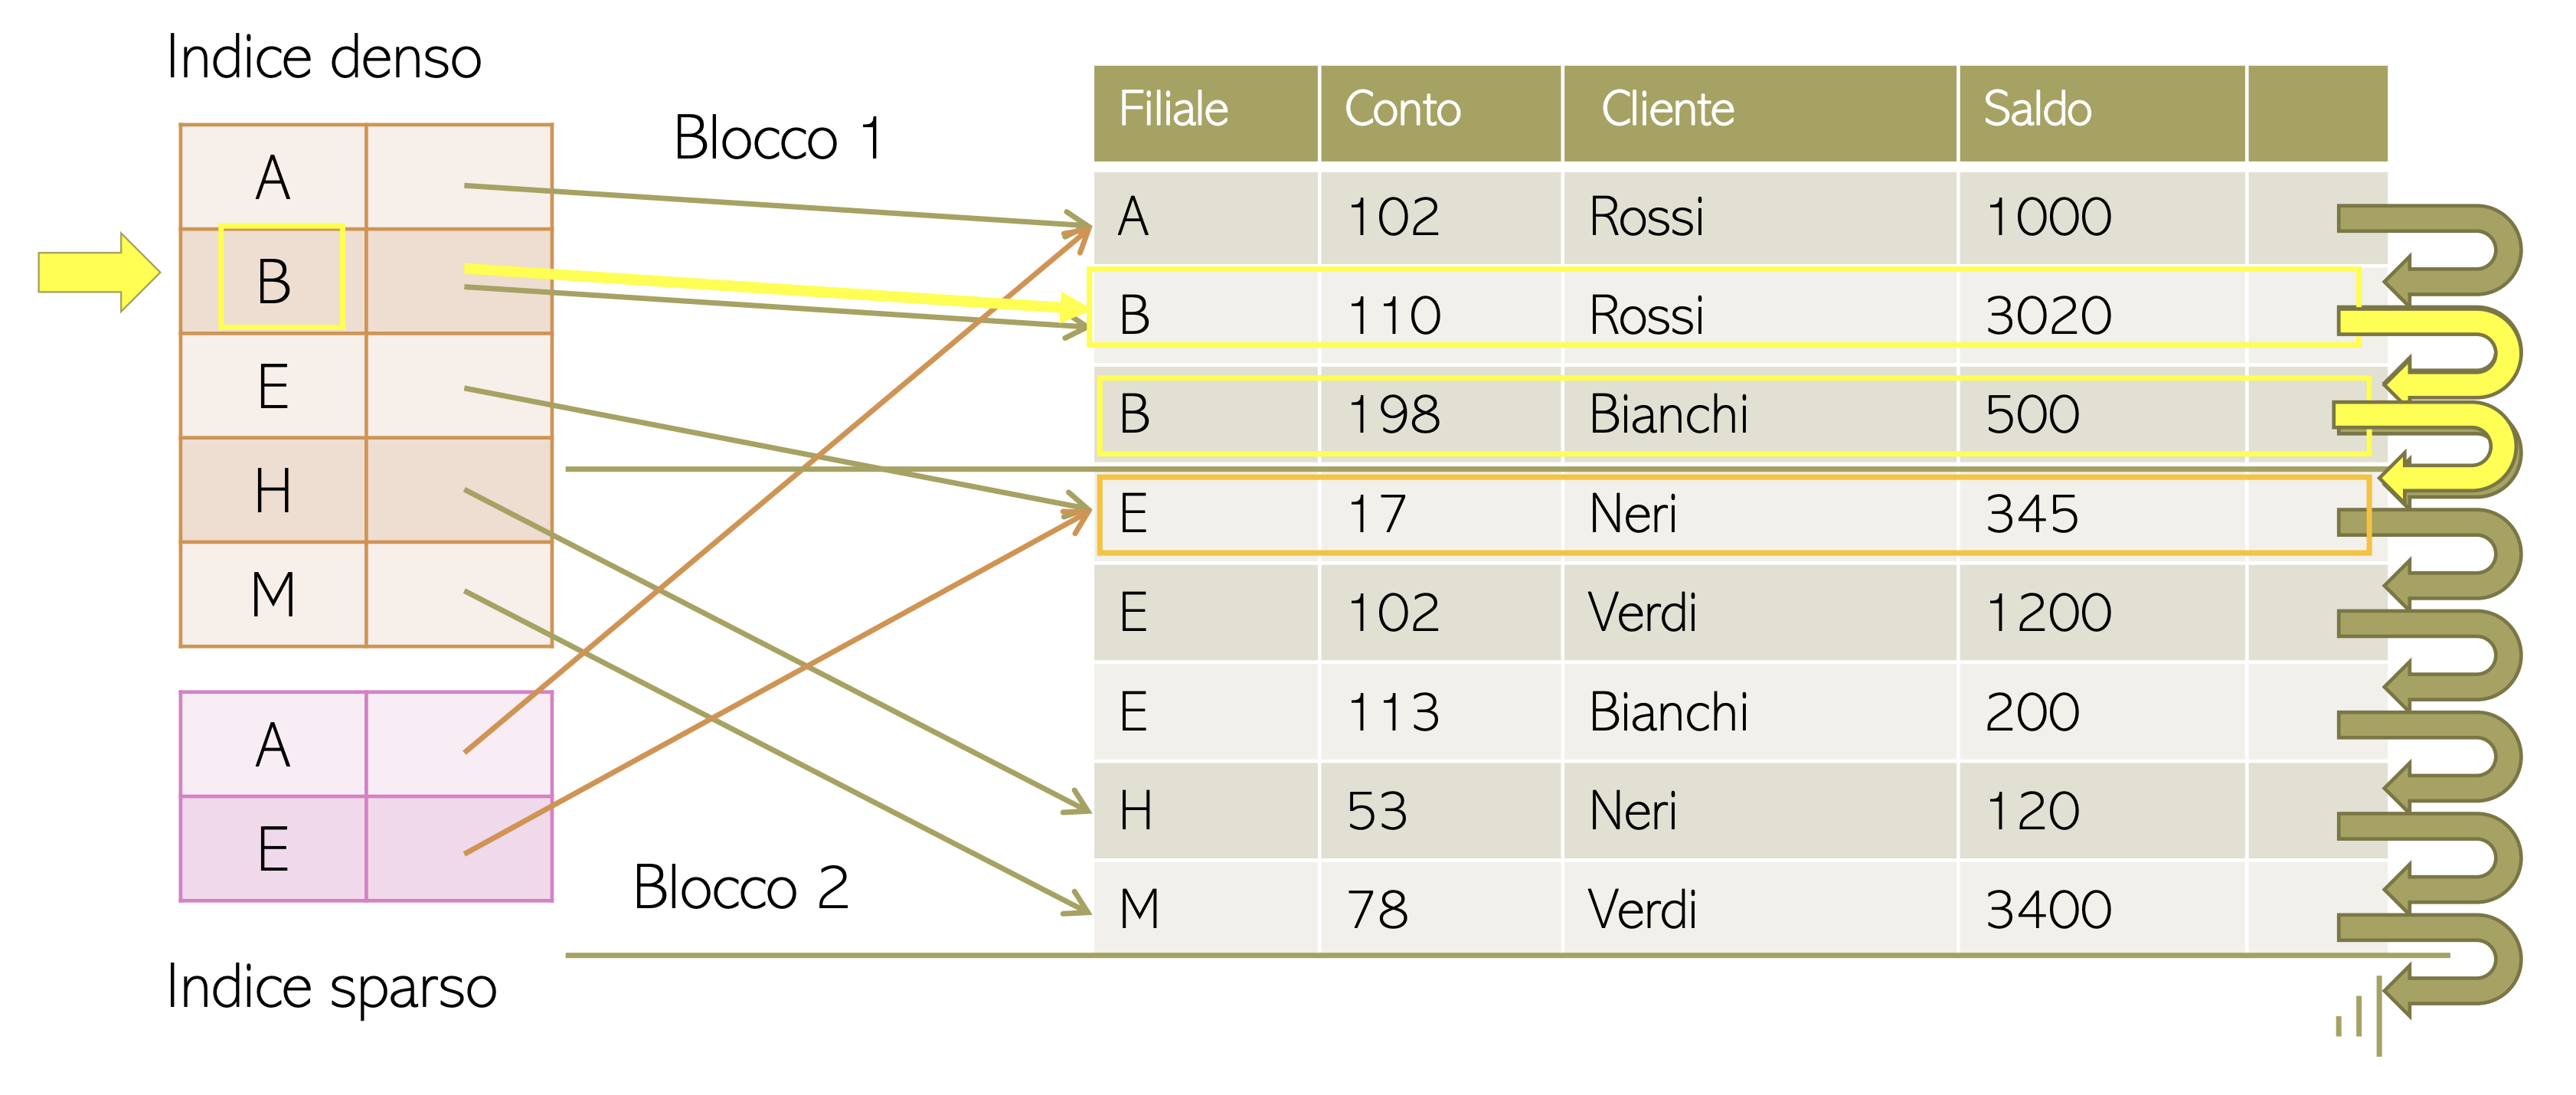
\includegraphics[width=0.6\textwidth]{images/indice-primario-denso.png}
          \caption{ricerca dei conti della filiale B}
        \end{figure}
      }

      \item se l'indice è sparso $\mathrm{K \rightarrow}$ potrebbe non essere presente nell'indice
      \begin{enumerate}[itemsep=\smallskipamount]
        \item scansione sequenziale dell'indice fino al record $\mathrm{(K', p_k)}$, dove $\mathrm{K'}$ è il valore più grande che sia minore o uguale a $\mathrm{K}$
        \item accesso al file attraverso il puntatore $\mathrm{p_k}$ e scansione del file (blocco corrente) per trovare le tuple con chiave $\mathrm{K}$
      \end{enumerate}

      $\Rightarrow$ \hl{\textbf{costo}: 1 accesso indice + 1 accesso blocco dati}

      \esempio{ricerca con indice primario sparso}{
        Un esempio di ricerca con indice primario sparso è il seguente:
        \begin{figure}[H]
          \centering
          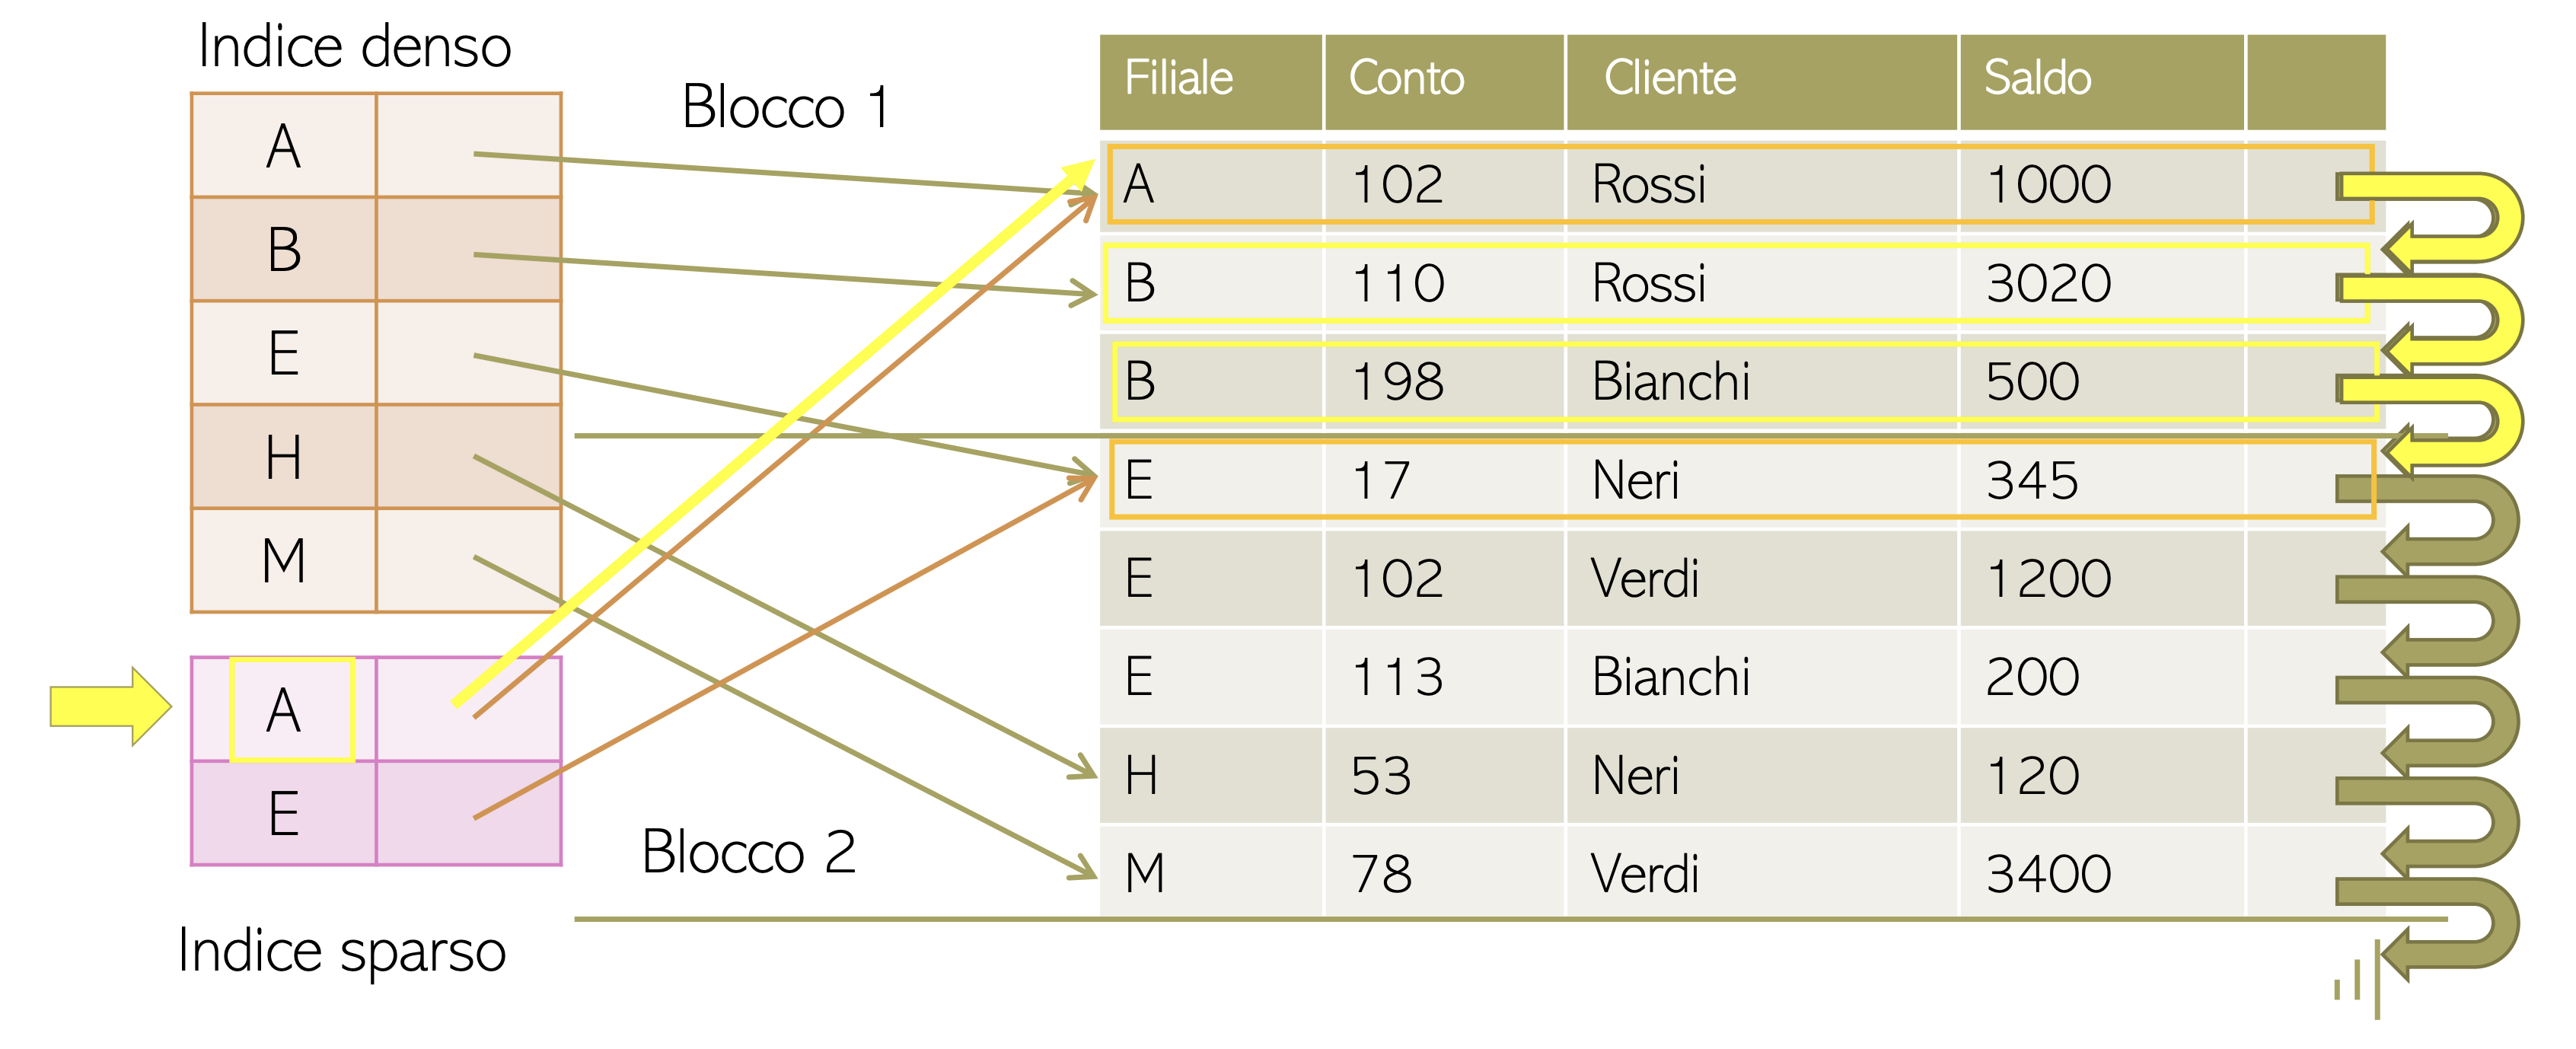
\includegraphics[width=0.6\textwidth]{images/indice-primario-sparso.png}
          \caption{ricerca dei conti della filiale B}
        \end{figure}
      }
    \end{itemize}

    \item \textbf{inserimento di un record nell'indice}
    \begin{itemize}[label=$\circ$, itemsep=\smallskipamount]
      \item \textbf{indice è denso}: inserimento nell'indice avviene solo se la tupla inserita nel file ha un valore di chiave K che non è già presente
      \item \textbf{indice è sparso}: inserimento avviene solo quando, per effetto dell'inserimento di una nuova tupla, si aggiunge un blocco dati alla struttura (negli altri casi rimane invariato)
    \end{itemize}

    \smallskip
    Gli indici sono costosi, quindi, bisogna fare un compromesso sul numero di indici da mantenere e il numero di attributi ad accesso sequenziale.

  \item  \textbf{cancellazione} di un record nell’indice
  \begin{itemize}[label=$\circ$, itemsep=\smallskipamount]
    \item \textbf{indice è denso}: cancellazione nell'indice avviene solo se la tupla cancellata nel file è l'ultima tupla con valore di chiave $\mathrm{K}$
    \item \textbf{indice è sparso}: cancellazione nell'indice avviene solo quando $\mathrm{K}$ è presente nell'indice e il corrispondente blocco viene eliminato
    
    Nel caso in cui il blocco sopravvive, va sostituito $\mathrm{K}$ nel record dell'indice con il primo valore $\mathrm{K'}$ presente nel blocco.
  \end{itemize}
\end{itemize}
\item \textbf{indice secondario}: la chiave di ordinamento e la chiave di ricerca sono diverse.

Ogni record dell'indice secondario contiene una coppia $\mathrm{\langle v_i, p_i \rangle}$, dove:
\begin{itemize}
  \item $\mathrm{v_i}$: valore della chiave di ricerca
  \item $\mathrm{p_i}$: puntatore al bucket di puntatori che individuano nel file sequenziale tutte le tuple con chiave $\mathrm{v_i}$
\end{itemize}

Gli indici secondari sono sempre densi perchè non si può sfruttare l'ordinamento delle tuple.

Le operazioni che si possono eseguire su un indice secondario sono:
\begin{itemize}[label=$\diamond$, itemsep=\medskipamount]
  \item \textbf{ricerca di una tupla con chiave di ricerca} $\mathbf{K}$
  \begin{enumerate}[itemsep=\smallskipamount]
    \item scansione sequenziale dell'indice per trovare il record $\mathrm{(K, p_k)}$
    \item accesso al bucket $\mathrm{B}$ di puntatori attraverso il puntatore $\mathrm{B}$
    \item accesso al file attraverso i puntatori del bucket $\mathrm{B}$
  \end{enumerate}
  
  $\Rightarrow$ \hl{\textbf{costo}: 1 accesso indice + 1 accesso al bucket + n accessi alle pagine dati} (n è il numero di puntatori nel bucket B)

  \esempio{ricarca con indice secondario}{
    Un esempio di ricerca con indice secondarioè il seguente:
    \begin{figure}[H]
      \centering
      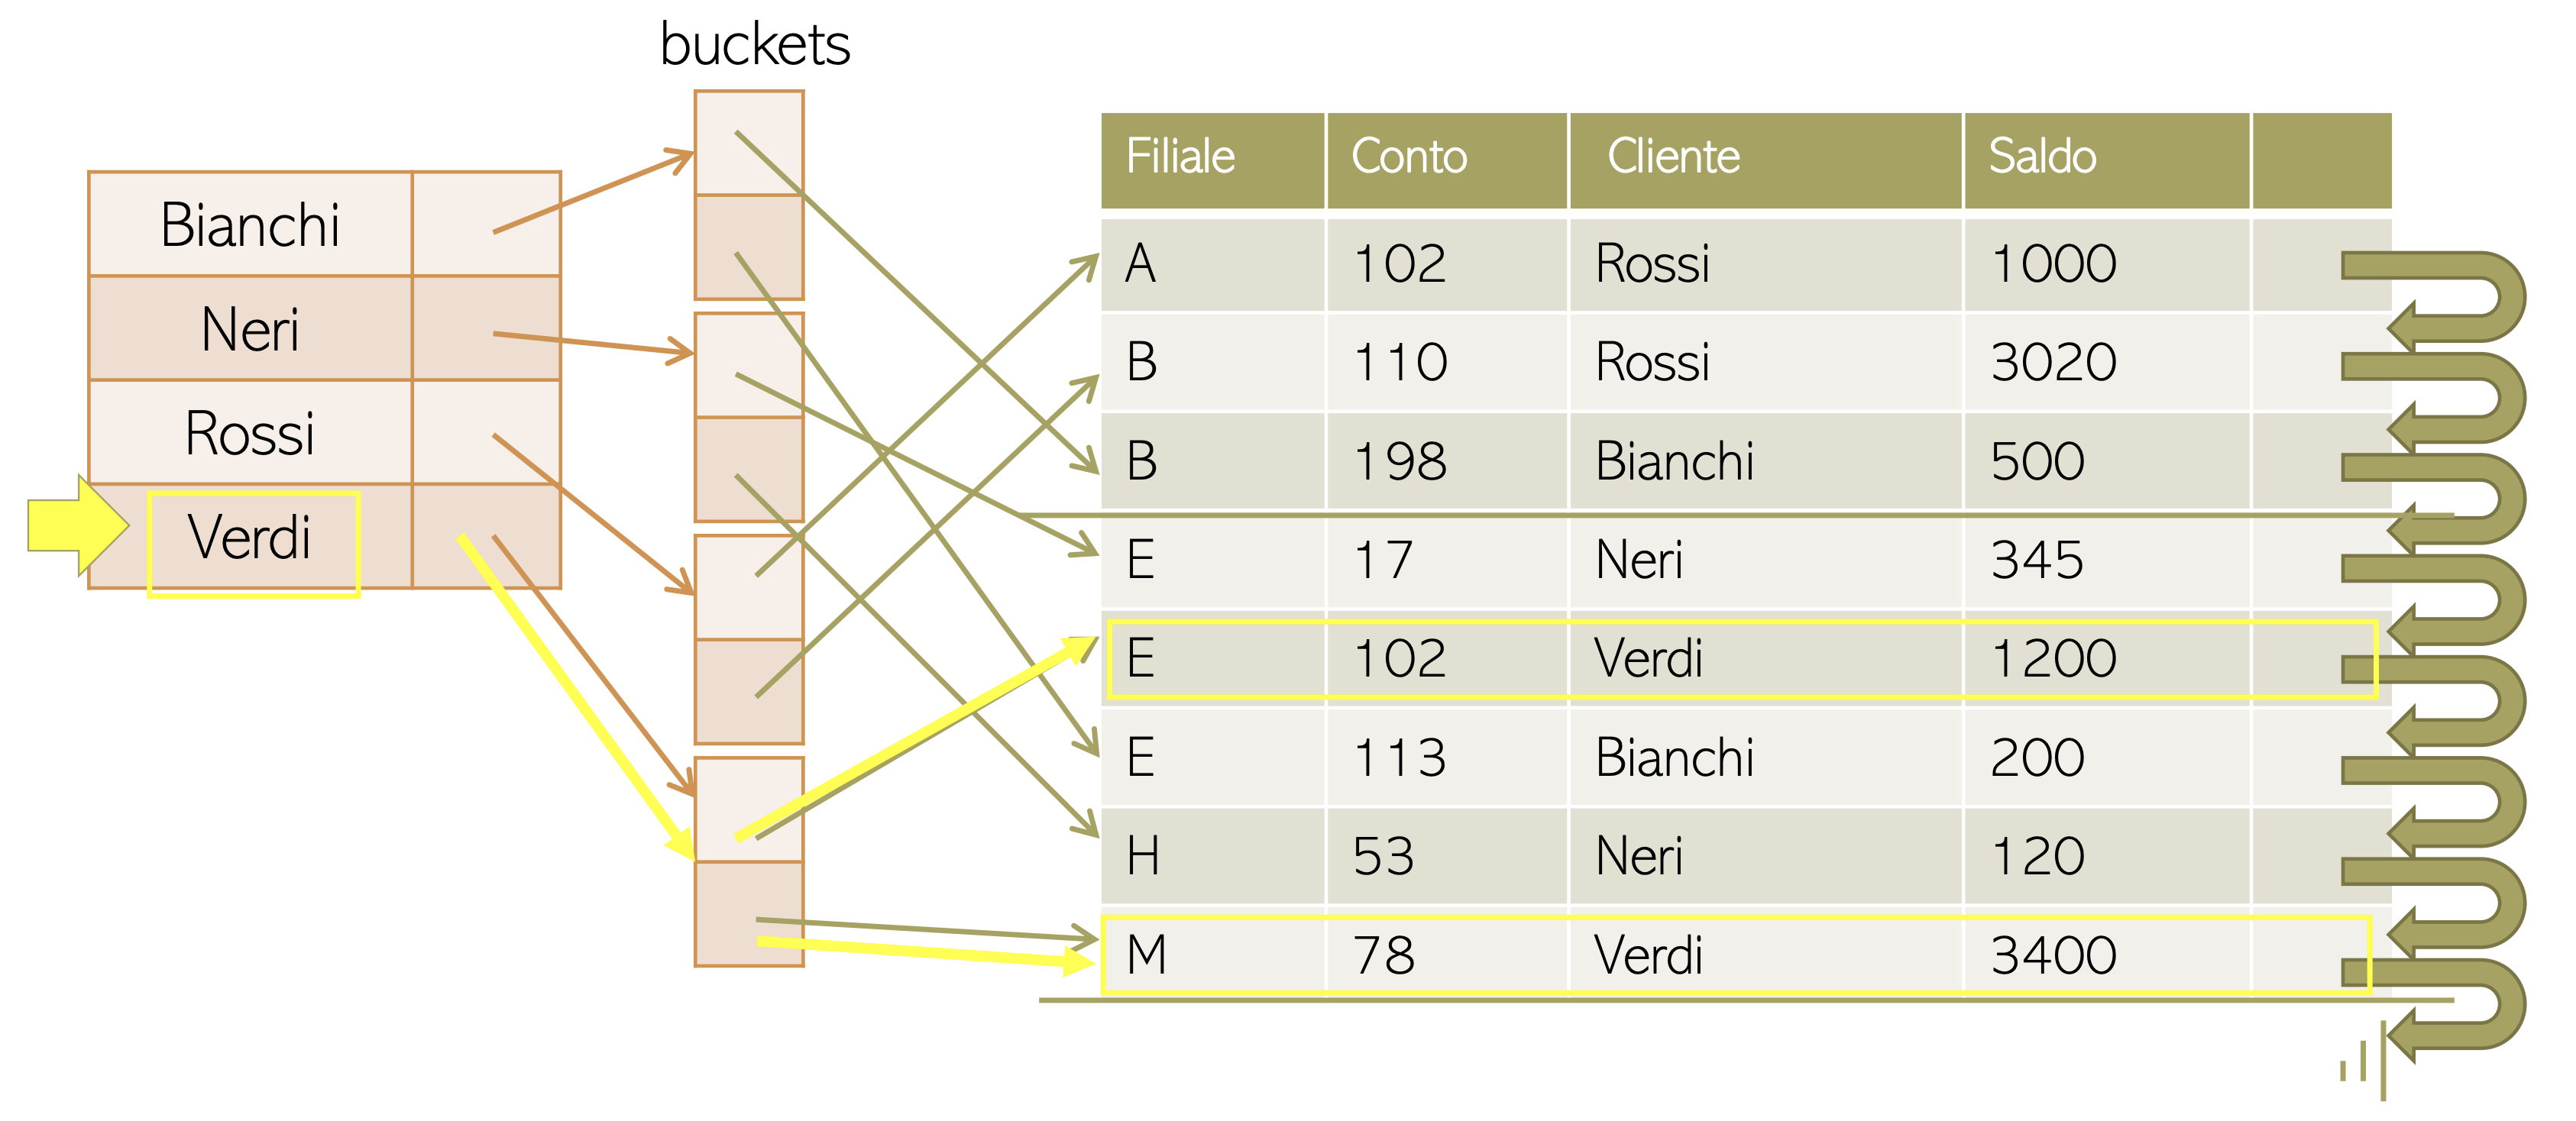
\includegraphics[width=0.6\textwidth]{images/indice-secondario.png}
      \caption{ricerca dei conti della filiale B}
    \end{figure}
  }

  \item  \textbf{inserimento} e \textbf{cancellazione}: si effettuano gli stessi passi dell'inserimento e della cancellazione in un indice primario denso, con in più l'aggiornamento dei bucket
\end{itemize}
\end{itemize}

\subsubsection{Struttura ad albero}
Quando l'indice aumenta di dimensioni non si può più gestire in memoria centrale, di conseguenza deve essere gestito in memoria secondaria.\\[0.2ex]
Per migliorare le prestazioni degli accessi a un indice di grandi dimensioni, si utilizza il $\verb|B+ tree|$, in cui:
\begin{itemize}[label=$\triangleright$, itemsep=\smallskipamount]
  \item ogni nodo viene memorizzato in una pagina della memoria secondaria
  \item legami tra nodi = puntatori a pagina
  \item sono presenti molti figli e di conseguenza ha pochi livelli
  \item albero bilanciato: la lunghezza dei percorsi che collegano la radice ai nodi foglia è costante
  \item inserimenti e cancellazioni non alterano le prestazioni dell'accesso ai dati: l'albero si mantiene bilanciato
\end{itemize}

\paragraph{Struttura}
La struttura di un $\verb|B+ tree|$ con fan-out = n (n figli per nodo) è la seguente:
\begin{itemize}[label=$\triangleright$, itemsep=\medskipamount]
  \item \textbf{nodo foglia}
  
  \begin{figure}[H]
    \centering
    \includegraphics[width=0.5\textwidth]{images/nodo-foglia-BTree.png}  
  \end{figure}

  Può contenere fino a $\mathbf{n - 1}$ valori ordinati di chiave di ricerca e fino a $\mathbf{n}$ puntatori ai dati.\\[0.2ex]
  Ogni nodo foglia ha un vincolo di ordinamento, cioè:
  \begin{itemize}[label=$\circ$, itemsep=\smallskipamount]
    \item chiavi dentro a un nodo foglia sono ordinate
    \item nodi foglia sono ordinati tra di loro.
    
    Dati due nodi foglia $\mathrm{L_i}$ e $\mathrm{L_j}$ con $\mathrm{i < j}$, allora:
    \begin{equation*}
      \mathrm{\forall k_i \in L_i; \quad \forall k_s \in L_j; \quad k_t < k_s}
    \end{equation*}
  \end{itemize}

  Il puntatore $\mathrm{p_m}$ del nodo $\mathrm{L_i}$ punta al nodo foglia $\mathrm{L_{i+1}}$ (se esiste):

  \begin{figure}[H]
    \centering
    \includegraphics[width=0.5\textwidth]{images/puntatore-nodo-foglia-BTree.png}
  \end{figure}

  Una variante del $\verb|B+ tree|$ è quella in cui i nodi foglia contengono direttamente le tuple.

  In questo caso si ha una struttura fisica integrata.


  \item \textbf{nodo intermedio}: è una sequenza di $\mathrm{m' \leq n}$ valori ordinati di chiave (può contenere fino a $\mathrm{n}$ puntatori a nodo).

  Ogni nodo chiave $\mathrm{K_i}$ è seguita da un puntatore $\mathrm{p_i}$:
  \begin{figure}[H]
    \centering
    \includegraphics[width=0.5\textwidth]{images/nodo-intermedio-BTree.png}
  \end{figure}
\end{itemize}

\paragraph{Vincoli di riempimento}
Il fan-out è un parametro che fornisce il limite massimo, ma bisogna anche fornire un limite minimo per evitare che i nodi siano troppo vuoti e sono chiamati \textbf{vincoli di riempimento}:
\begin{itemize}[label=$\diamond$, itemsep=\medskipamount]
  \item \textbf{vincoli per i nodi foglia}: ogni nodo foglia può contenere un numero di valori di chiavi ($\mathrm{\# \ chiavi}$) vincolato
  \begin{equation*}
    \mathrm{\left\lceil \frac{n - 1}{2} \right\rceil \leq \# \ chiavi \leq n - 1}
  \end{equation*}
  \item \textbf{vincoli per i nodi intermedi}: ogni nodo intermedio può contenere un numero di puntatori ($\mathrm{\# \ puntatori}$) vincolato
  \begin{equation*}
    \mathrm{\left\lceil \frac{n}{2} \right\rceil \leq \# \ puntatori \leq n}
  \end{equation*}
\end{itemize}

\esempio{utilizzo del \texttt{B+-tree}}{
  Consideriamo ad esempio un B+-Tree con fan-out = 4 con contenuto:
  \[
    \mathrm{A, B, D, E, F, G, L, M, N, P}
  \] 
  Il fan-out ci dice che per:
  \begin{itemize}
    \item \textbf{nodi foglia}: vincoli di riempimento sono
      \[
        2 \le \#chiavi \le 3
      \] 

    \item \textbf{nodi intermedi}: vincoli di riempimento sono
      \[
        2 \le \#puntatori \le 4
      \]

    \item \textbf{radice}: unico nodo per cui i vincoli di riempimento \textbf{minimi}
      non si applicano
  \end{itemize}
  \begin{figure}[H]
    \centering
    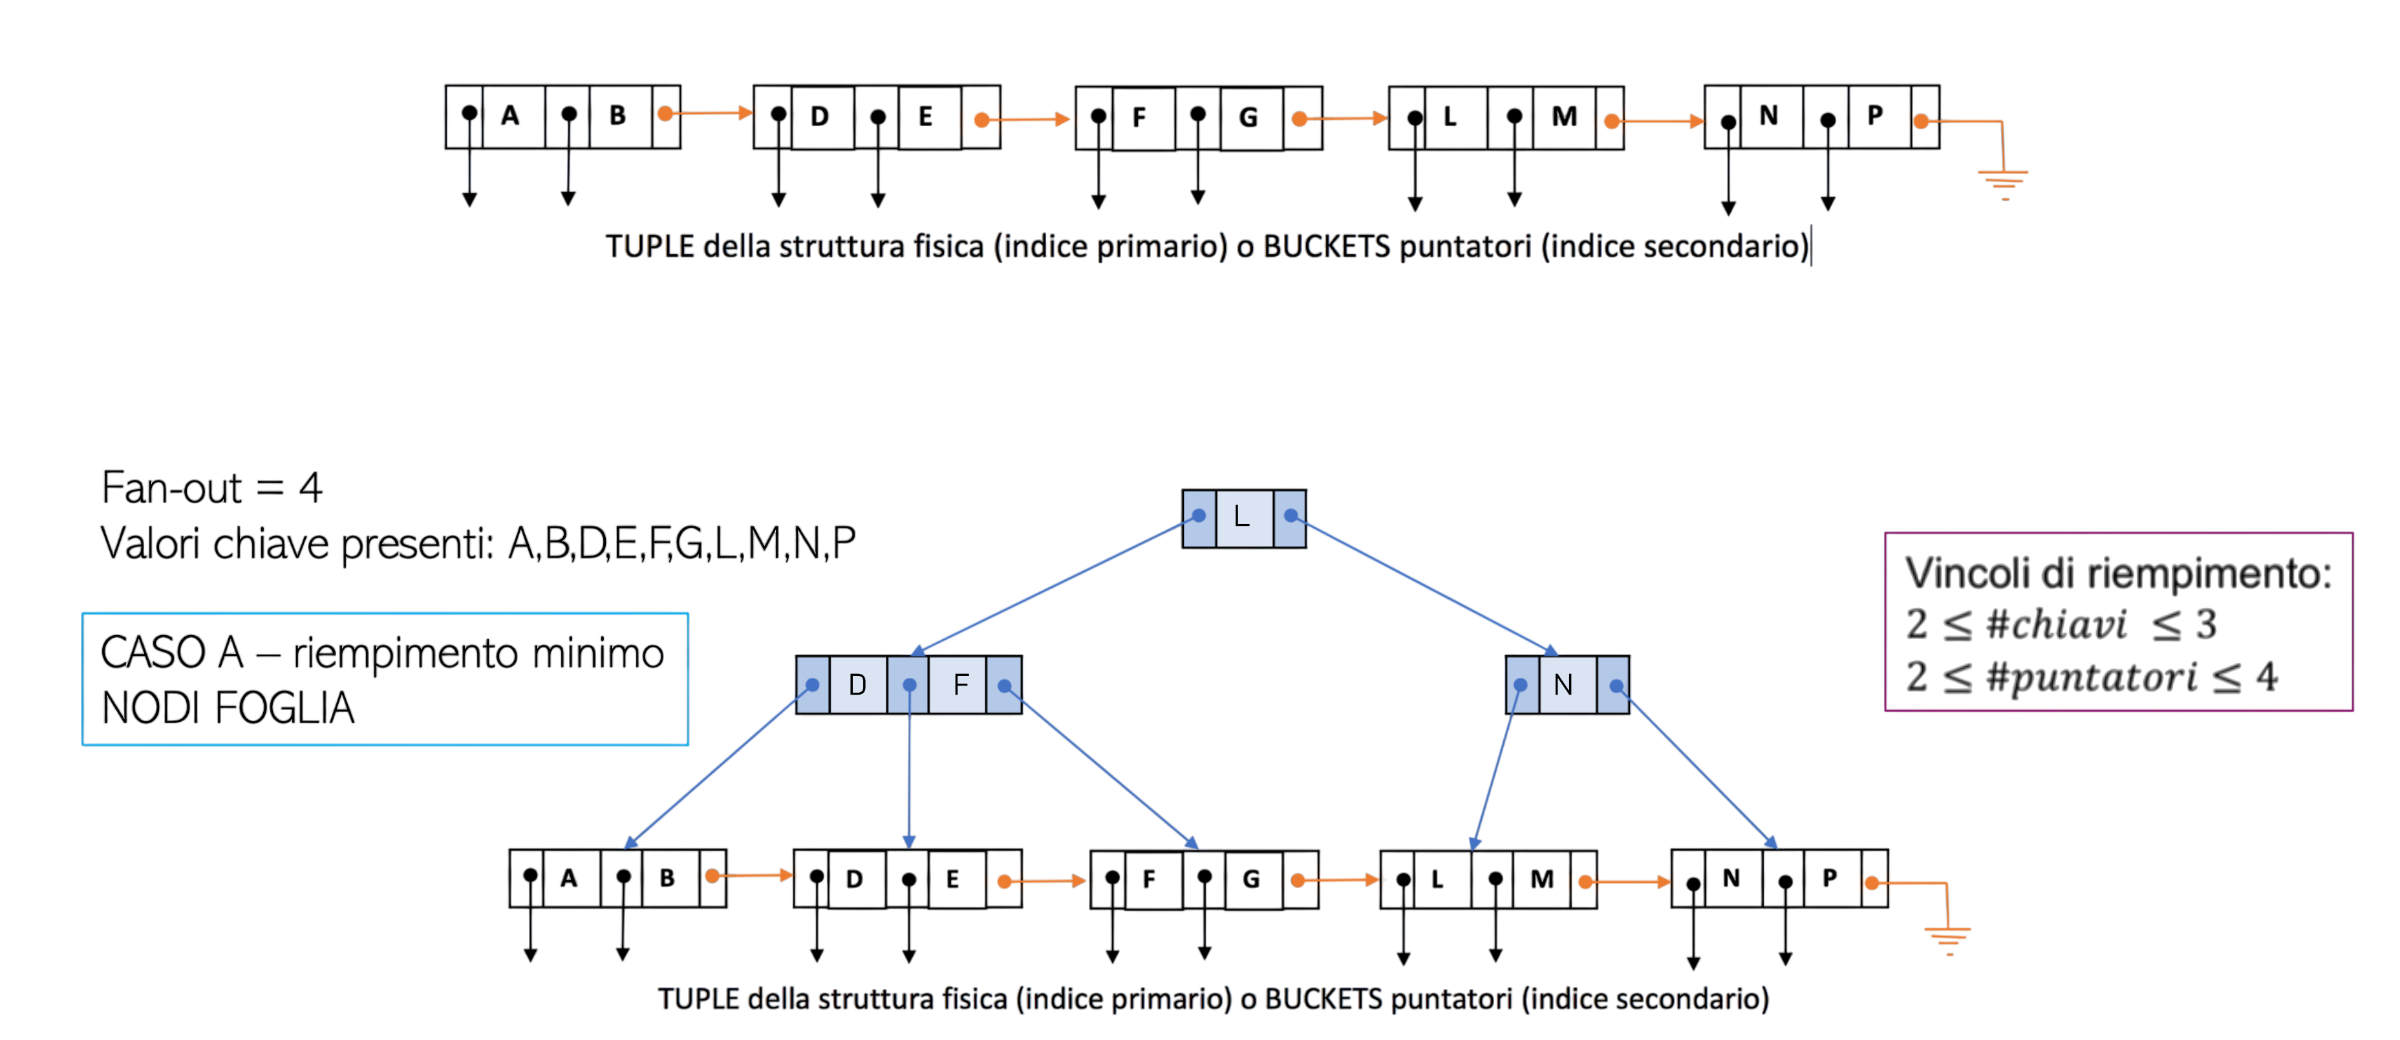
\includegraphics[width=0.8\textwidth]{images/b_plus_tree_esempio.png}
    \caption{Esempio di B+-Tree con vincolo di riempimento minimo}
  \end{figure}

  La radice \( \mathrm{L} \) punta:
  \begin{itemize}[label=$\diamond$, itemsep=\smallskipamount]
    \item a sinistra: al sottoalbero con chiave \( \mathrm{K < "L"} \) 
    \item a destra: al sottoalbero con chiave \( \mathrm{K \ge "L"} \)
  \end{itemize}

  \smallskip
  I figli puntano alle tuple con chiave uguale a quella del nodo foglia.
  
  In questo caso l'albero per chiavi desiderate rispetta il vincolo di riempimento minimo.
  
  Per rispettare il vincolo di riempimento massimo bisogna fare un altro albero:
  \begin{figure}[H]
    \centering
    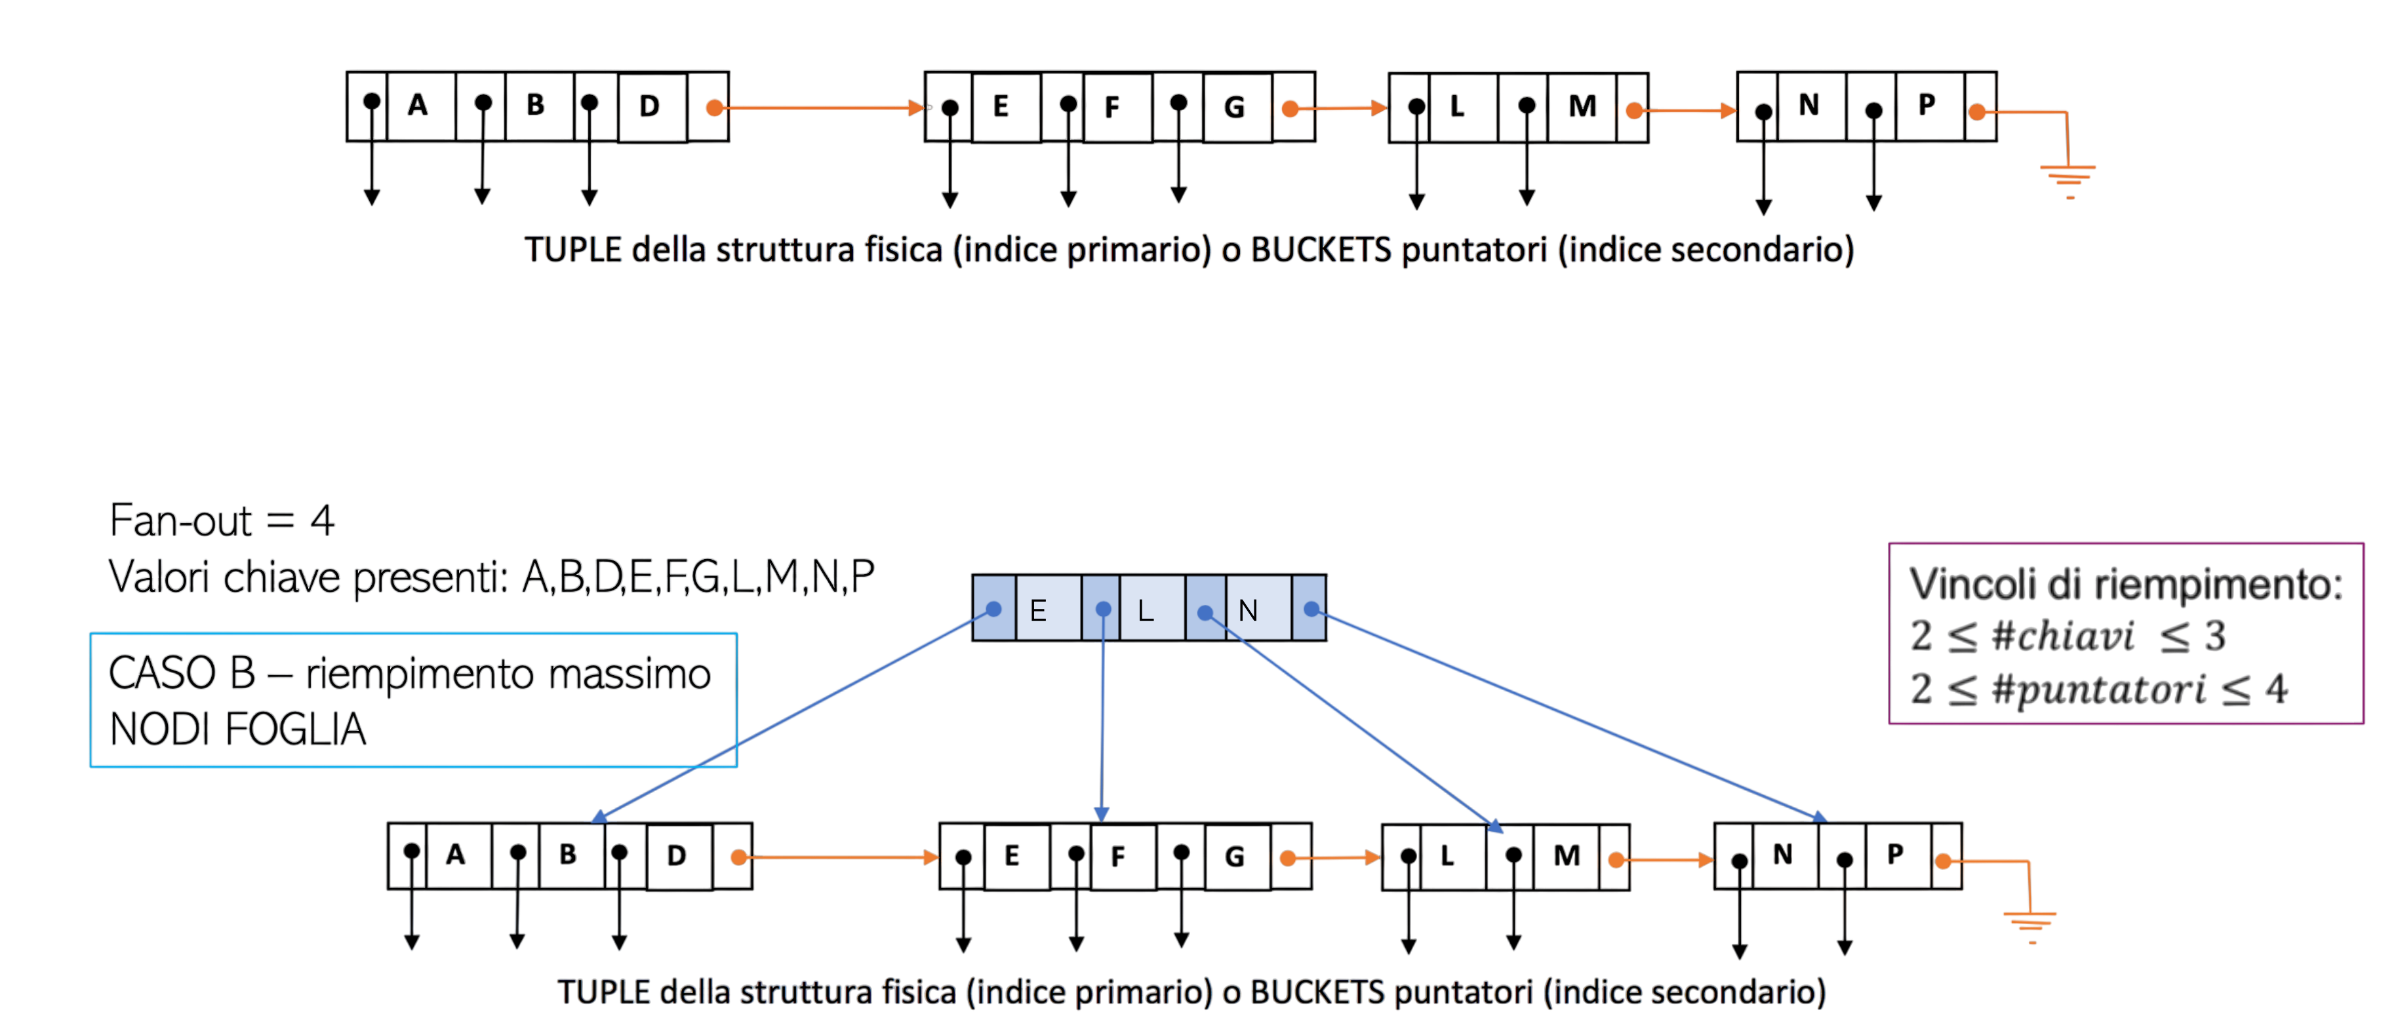
\includegraphics[width=0.8\textwidth]{images/b_plus_tree_esempio2.png}
    \caption{Esempio di B+-Tree con vincolo di riempimento massimo}
  \end{figure}

  Le etichette per la radice sono assegnate secondo:
  \begin{itemize}[label=$\circ$, itemsep=\smallskipamount]
    \item sinistra: Chiavi comprese tra: \( \mathrm{"E" \le K < "L"} \) 
    \item centro: Chiavi comprese tra \( \mathrm{"L" \le K < "N"} \)
    \item destra: Chiavi \( \mathrm{K \ge "N"} \)
  \end{itemize}
}

\paragraph{Operazione: ricerca con chiave K}
Per effettuare la ricerca di una tupla con chiave di ricerca K si effettuano i seguenti passi:
\begin{enumerate}[itemsep=\medskipamount]
  \item \textbf{cercare nel nodo radice il più piccolo valore di chiave maggiore di K}
  \begin{itemize}[label=$\triangleright$, itemsep=\medskipamount]
    \item se il valore esiste ($\mathrm{value = k_i}$) $\rightarrow$ seguire il puntatore $\mathrm{p_i}$
    \begin{figure}[H]
      \centering
      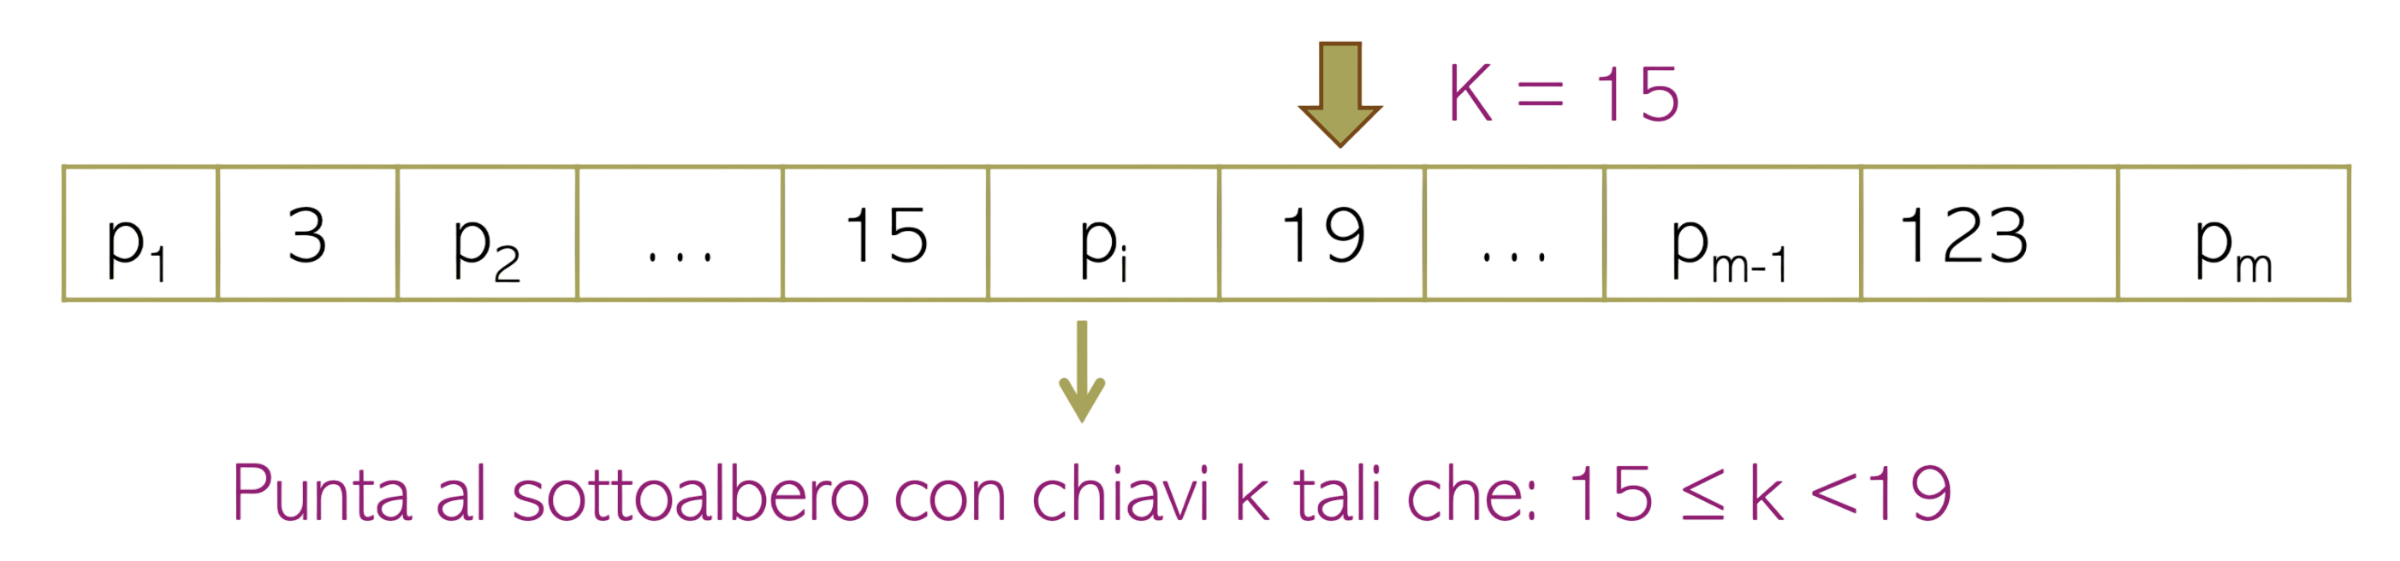
\includegraphics[width=0.5\textwidth]{images/ricerca-chiave-k-nodoRadice1.png}
    \end{figure}
    \item se il valore non esiste $\rightarrow$ seguire puntatore $\mathrm{p_m}$
    \begin{figure}[H]
      \centering
      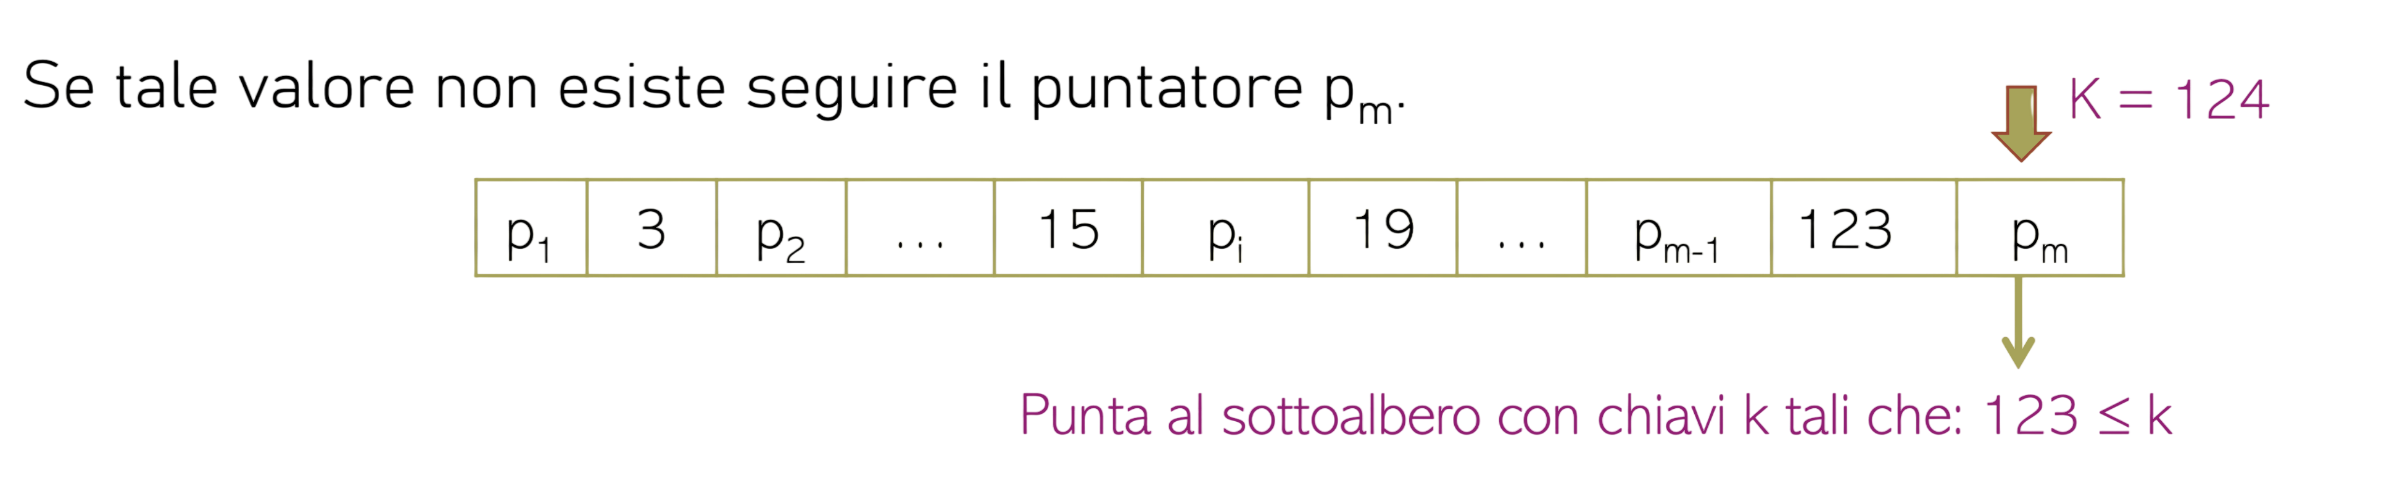
\includegraphics[width=0.5\textwidth]{images/ricerca-chiave-K-nodoRadice2.png}
    \end{figure}
  \end{itemize}
  \item \textbf{cercare il valore K (se nodo raggiunto = nodo foglia) e seguire il corrispondente puntatore verso le tuple} o \textbf{riprendere il passo 1 (se non esistono)}
  \begin{figure}[H]
    \centering
    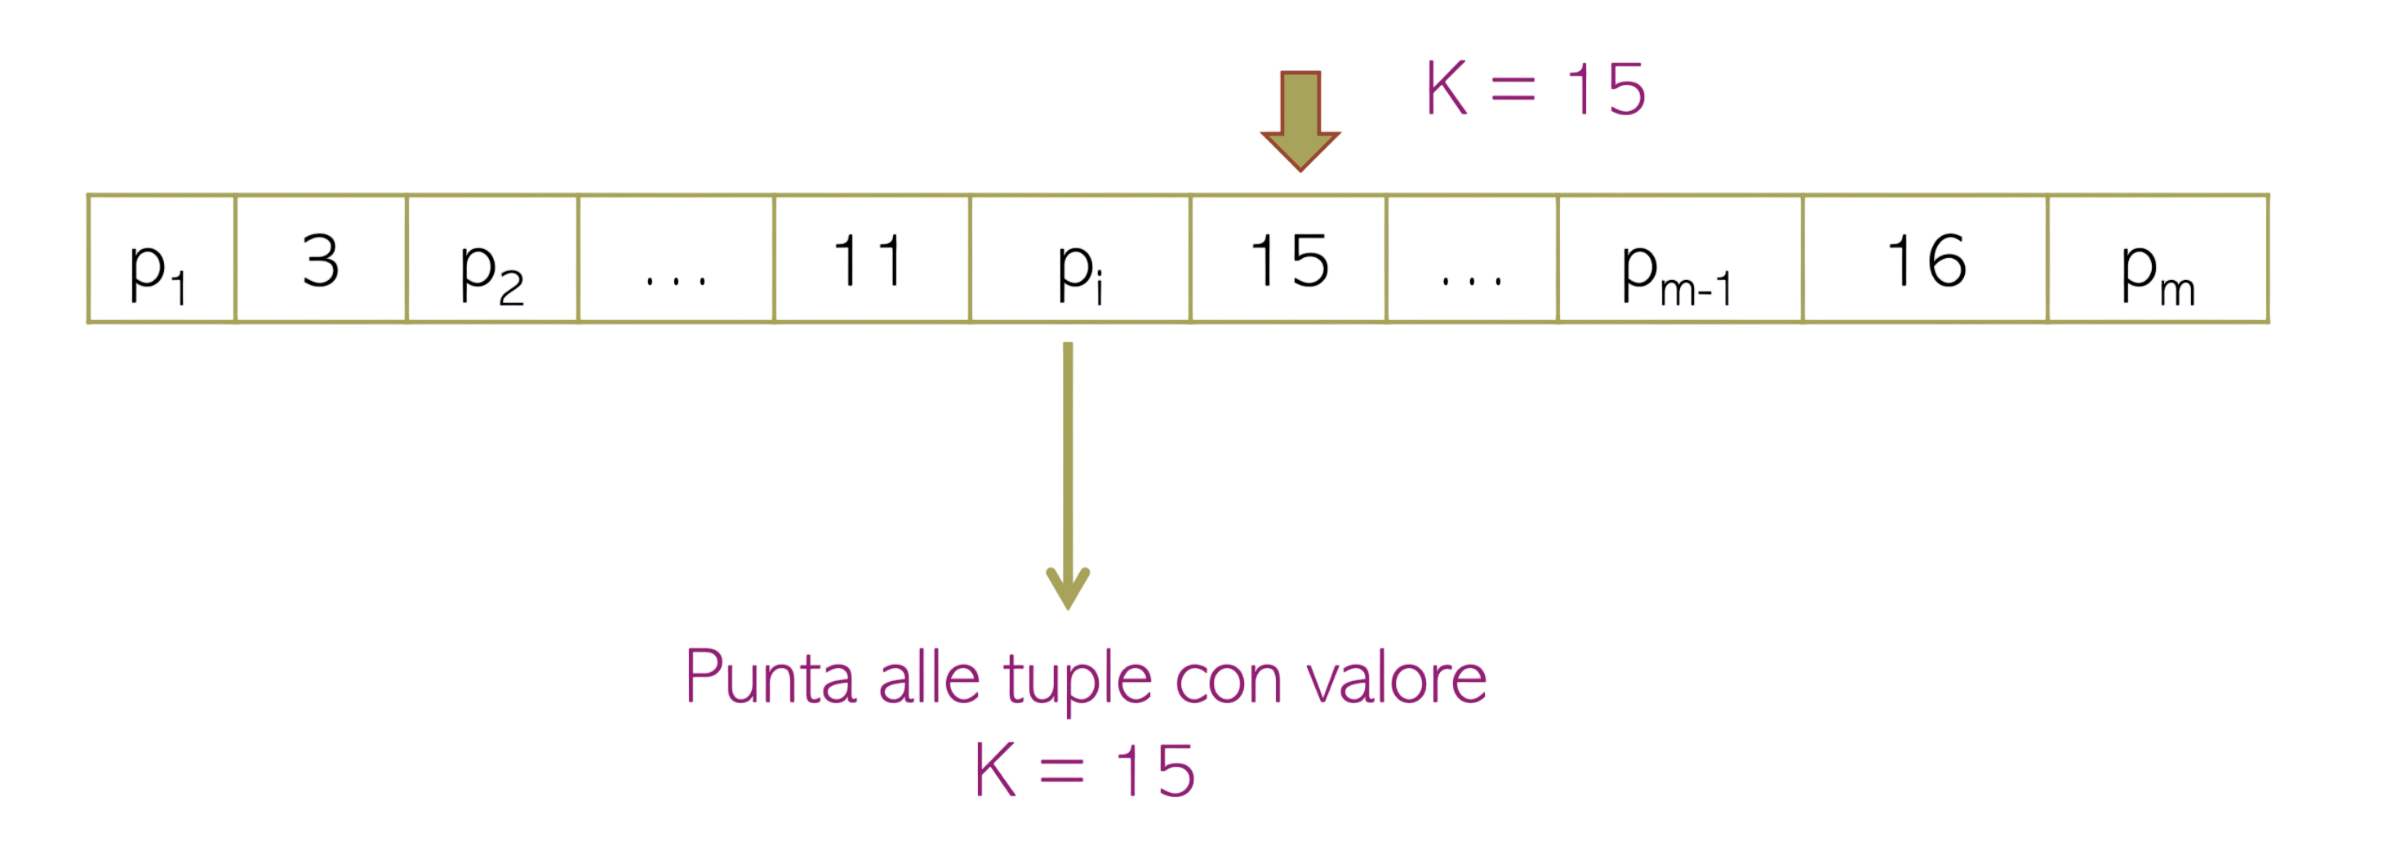
\includegraphics[width=0.5\textwidth]{images/ricerca-chiave-k-nodoFoglia.png}
  \end{figure}
\end{enumerate}

\esempio{ricerca di una tupla con chiave di ricerca K = "G"}{
  \begin{figure}[H]
    \centering
    \includegraphics[width=1.0\textwidth]{images/esempio-ricerca-chiave-k.png}
  \end{figure}
}

Il costo della ricerca dipende dalla profondità dell'albero in termini di \textbf{accessi alla memoria secondaria}, dove ogni metodo rappresenta un blocco.\\[0.2ex]
Il \underline{costo in una struttura ad albero} è pari alla profondità dell'albero, che nel $\verb|B+ tree|$ è indipendente dal percorso ed è funzione del fan-out $\mathrm{n}$ e del numero di valori di chiave presente nell'albero $\mathrm{\# \ valoriChiave}$.
\begin{equation*}
  \mathrm{prof_{B+ tree}} \leq \underbrace{1}_{\text{radice}} + \underbrace{\log_{\left\lceil \frac{n}{2} \right\rceil} \left( \frac{\overbrace{\# \text{valoriChiave}}^{\text{nodi foglia massimi}}}{\left\lceil \frac{n - 1}{2} \right\rceil} \right)}_{\text{\# livelli}}
\end{equation*}

\paragraph{Operazione: inserimento}
Per inserire una tupla in un $\verb|B+ tree|$ bisogna mantenere i vincoli di riempimento, quindi, vengono eseguiti i seguenti passi:
\begin{enumerate}[itemsep=\medskipamount]
  \item \textbf{ricerca del nodo foglia NF dove K va inserito}
  \item 
  \begin{itemize}[label=$\triangleright$, itemsep=\medskipamount]
    \item se K è presente in NF:
    \begin{itemize}[label=$\diamond$, itemsep=\smallskipamount]
      \item se è \textbf{indice primario} $\rightarrow$ non si fa nessuna azione
      \item se è \textbf{indice secondario} $\rightarrow$ si aggiornano i bucket dei puntatori
    \end{itemize}
    \item se k non è prensente in NF:
    \begin{itemize}[label=$\diamond$, itemsep=\smallskipamount]
      \item se è \textbf{indice primario} $\rightarrow$ si inserisce K e si aggiorna il puntatore alla prima tupla
      \item se è \textbf{indice secondario} $\rightarrow$ si inserisce K e si crea il bucket
    \end{itemize}
  \end{itemize}
  Se all'inserimento di K viene violato il vincolo di riempimento massimo, bisogna eseguire uno \textbf{split} del nodo NF in due nodi foglia.

  Lo split viene eseguito se in NF esistono già $\mathrm{n}$ valori di chiave e bisogna eseguire i seguenti passi:
  \begin{enumerate}[itemsep=\smallskipamount]
    \item creare due nodi foglia $\mathrm{NF_1}$ e $\mathrm{NF_2}$
    \item inserire i primi $\left\lceil \frac{n - 1}{2} \right\rceil$ valori di chiave in $\mathrm{NF_1}$
    \item inserire i restanti in $\mathrm{NF_2}$
    \item aggiornare il padre, cioè se il padre viola il vincola di riempimento massimo bisogna propogare lo split e, quindi, creare una nuova radice/livello se necessario 
  \end{enumerate}
\end{enumerate}

\esempio{split di un nodo foglia}{
  Lo split di un nodo foglia con fan-out = 5 è il seguente:

  \begin{figure}[H]
    \centering
    \includegraphics[width=0.9\textwidth]{images/split-nodo-foglia.png}
  \end{figure}

  Se si aggiungesse la chiave 15 tra il 12 e il 16 si violerebbe il vincolo di riempimento massimo: $\mathrm{\# \ chiavi = 5}$, quindi, si esegue lo split del nodo foglia.
}

\paragraph{Operazione: cancellazione}
Per cancellare una tupla in un $\verb|B+ tree|$ con chiave K bisogna mantenere i vincoli di riempimento, quindi, vengono eseguiti i seguenti passi:
\begin{enumerate}[itemsep=\medskipamount]
  \item \textbf{ricercare il nodo foglio NF che contiene K}
  \item \textbf{cancellare K e il suo puntatore}
  
  Potrebbe violare il vincolo di riempimento minimo, in quel caso bisogna fare il merge di NF con un fratello.

  Per fare il merge, se nel nodo da unire esistono $\left\lceil \frac{n - 1}{2} \right\rceil - 1$ valori chiavi, si procede:
  \begin{enumerate}[itemsep=\smallskipamount]
    \item individuare il nodo fratello
    \item generare un unico nodo foglia
    \item aggiornare il padre:
    \begin{itemize}[label=$\triangleright$, itemsep=\smallskipamount]
      \item se non c'è un nodo foglia fratello che unito rispetta il vincolo di riempimento massimo, si fa prima il merge e poi lo split
      \item se anche il padre viola il vincolo di riempimento massimo, si propaga il merge fino ad arrivare alla radice
    \end{itemize}
  \end{enumerate} 
\end{enumerate}

\esempio{merge di un nodo foglia}{
  Un esempio di merge di un nodo foglia con fan-out = 5, in cui si vuole eliminare la tupla con chiave K = "3" è il seguente:

  \begin{figure}[H]
    \centering
    \includegraphics[width=0.9\textwidth]{images/merge-nodo-foglia.png}
  \end{figure}

  Se si eliminasse il nodo con chiave 3 si violerebbe il vincolo di riempimento minimo, quindi, si deve fare il merge con il nodo fratello.
}

\subsubsection{Struttura ad accesso calcolato (hash)}
Questra struttura garantisce un \textbf{accesso associativo} alle tuple, cioè la locazione fisica dei dati dipende dal valore assunto dalla chiave.\\[0.2ex]
Si potrebbe utilizzare un array indicizzato dalla chiave, ma questo non è pratico perchè i valori della chiave sono tanti, quindi, si utilizza una \textbf{funzione di hash} che mappa i valori di chiave in indirizzi di memorizzazione delle tuple:
\begin{equation*}
  \mathbf{h : K \rightarrow B}
\end{equation*}

dove:
\begin{itemize}[label=$\triangleright$, itemsep=\smallskipamount]
  \item $\mathrm{K}$: dominio delle chiavi
  \item $\mathrm{B}$: dominio degli indirizzi di memorizzazione
\end{itemize}

Il vantaggio di questa struttura è che il costo della ricerca è costante e uguale a un accesso alla memoria secodaria.\\[0.2ex]
Lo svantaggio è quello delle \textbf{collisioni}, cioè valori di chiavi diversi possono produrre lo stesso indirizzo.\\[0.2ex]
Una funzione di hash \textbf{buona} minimizza il numero di collisioni.

\definizione{fattore riempimento}{
  Il \textbf{fattore riempimento} definisce la frazione di spazio fisico utilizzata da un blocco.
}

Siano:
\begin{itemize}[label=$\triangleright$, itemsep=\smallskipamount]
  \item $\mathrm{T}$: numero di tuple
  \item $\mathrm{F}$: fattore blocco (numero di tuple che ci stanno in un blocco)
  \item $\mathrm{f}$: fattore di riempimento
\end{itemize}

si ha che il numero di blocchi è definito come:
\begin{equation*}
  \boldsymbol{\mathrm{\# B = \left\lceil \frac{T}{F \cdot f} \right\rceil}}
\end{equation*}

Il DBMS alloca un numero di bucket di puntatori uguale al numero di blocchi $\mathrm{\# B}$.

Si definiscono due funzioni:
\begin{itemize}[label=$\diamond$, itemsep=\medskipamount]
  \item \textbf{funzione di folding}: trasforma i valori di chiave in numeri interi positivi
  \begin{equation*}
    \mathrm{f: K \rightarrow \mathbb{Z}^+}
  \end{equation*}
  \item \textbf{funzione di hashing}:
  \begin{equation*}
    \mathrm{h: \mathbb{Z}^+ \rightarrow B}
  \end{equation*}
\end{itemize}

\esempio{tabella di hash}{
  Un esempio di tabella di hash è il seguente:

  \begin{figure}[H]
    \centering
    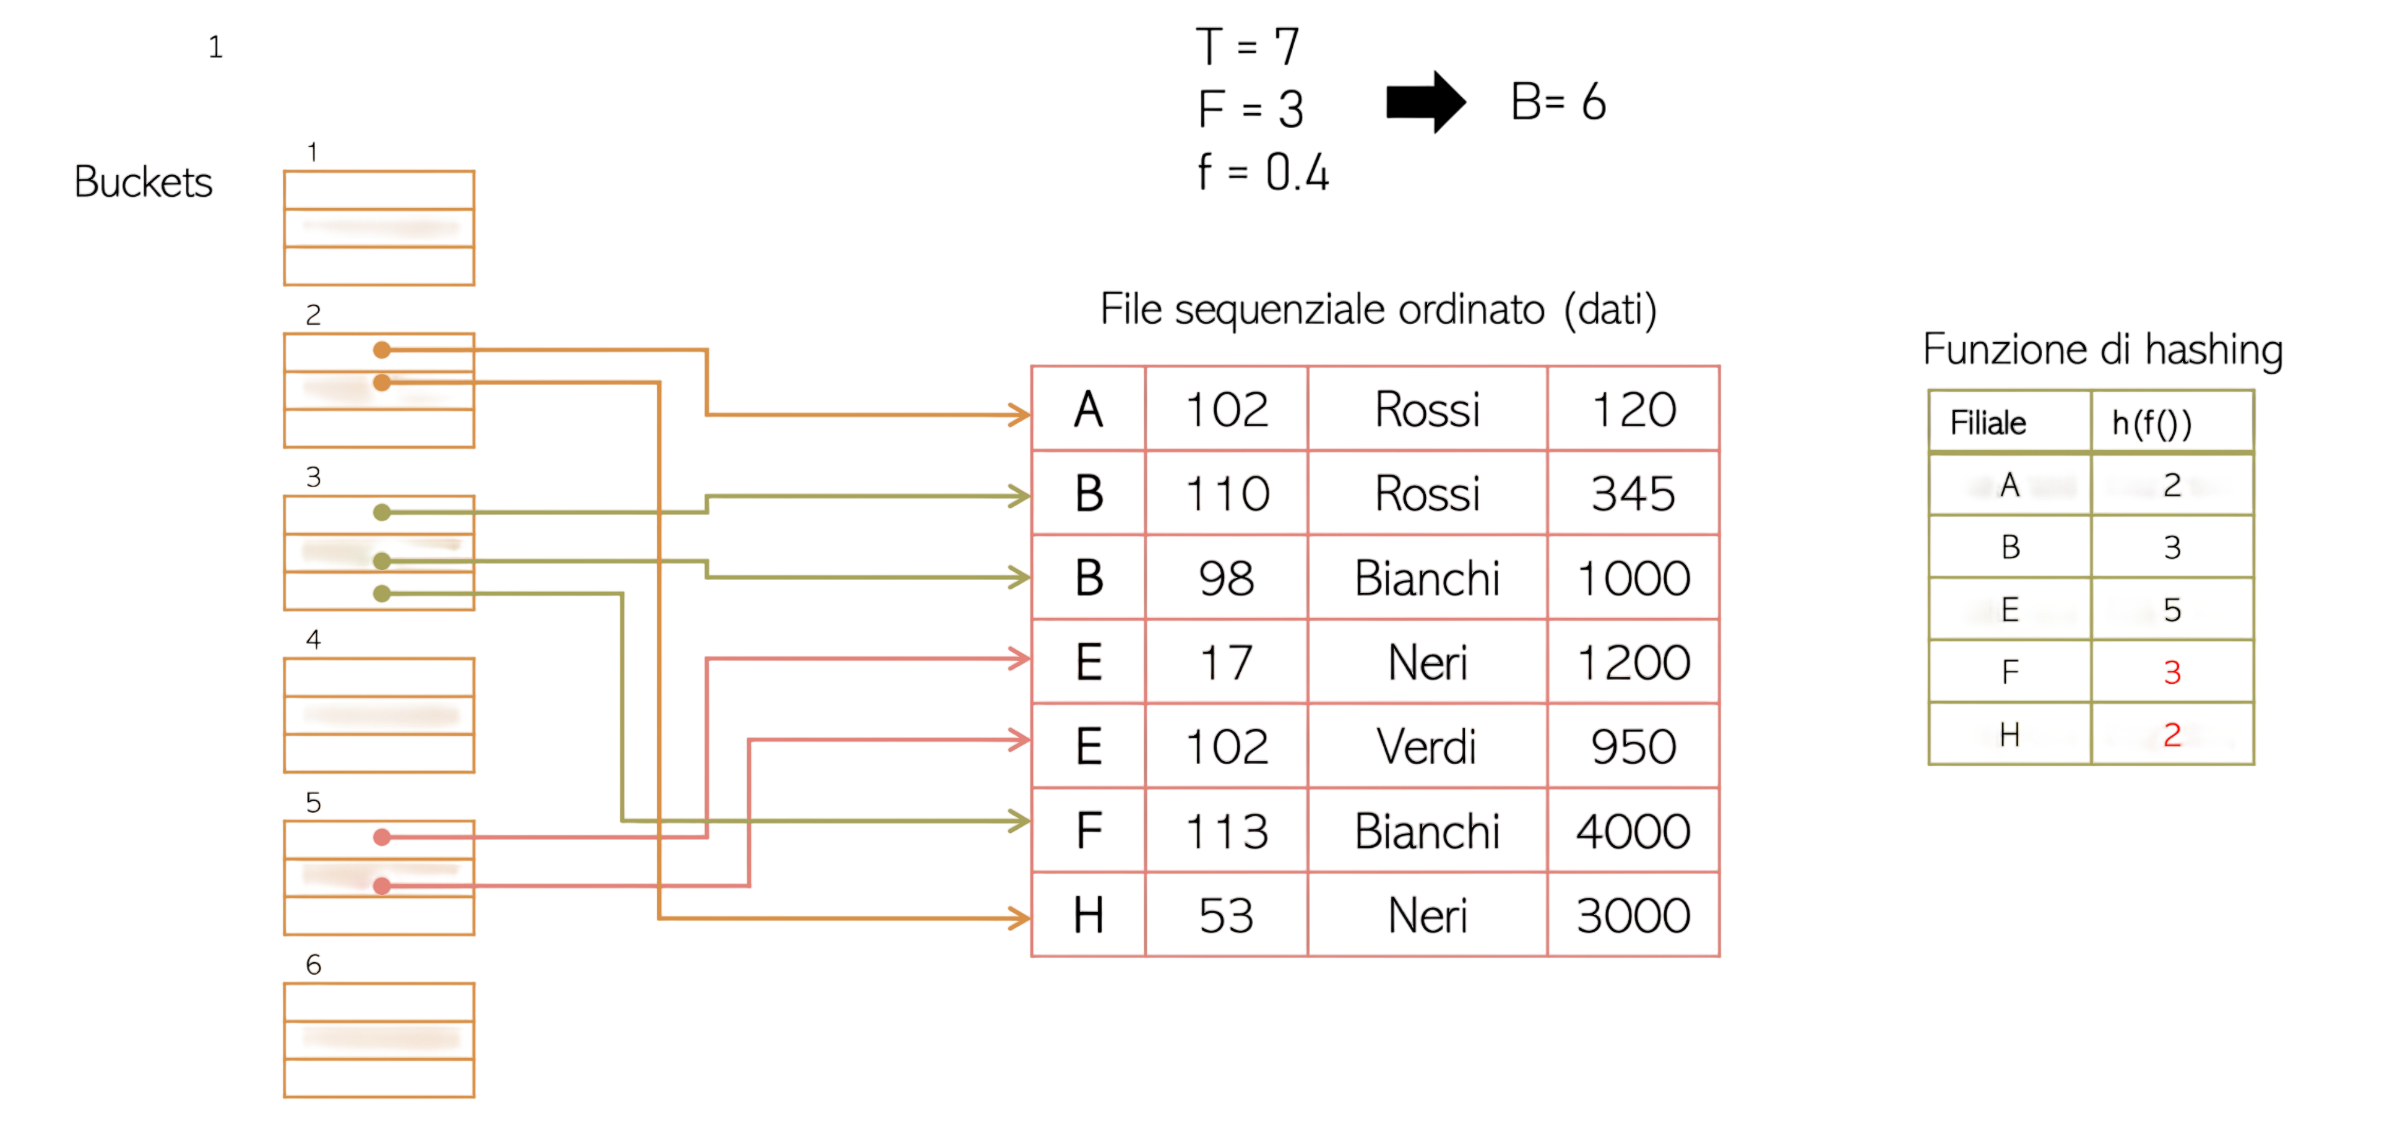
\includegraphics[width=0.9\textwidth]{images/esempio-tabella-hash.png}
  \end{figure}
}

\paragraph{Operazione: ricerca con chiave K}
Per efettuare la ricerca di una tupla con chiave di ricerca K si effettuano i seguenti passi:
\begin{enumerate}[itemsep=\medskipamount]
  \item calcolare $\mathrm{b = h(f(K))}$ (costo zero)
  \item accedere al bucket $\mathrm{b}$ (costo: 1 accesso alla pagina di memoria secondaria)
  \item accedere alle $\mathrm{n}$ tuple attraverso i puntatori del bucket (costo: $\mathrm{m}$ accessi a pagine di memoria secondaria, con $\mathrm{m \leq n}$)
\end{enumerate}

L'inserimento e la cancellazione hanno costo simile alla ricerca.

\paragraph{Collisioni}
La struttura ad accesso calcolato funziona se i buckets conservano un basso coefficiente di riempimento.\\[0.2ex]
Infatti, il problema delle strutture ad accesso calcolato è la gestione delle collisioni.

\definizione{collisione}{
  Una \textbf{collisione} si verifica, quando, dati due valori di chiave $\mathrm{K_1}$ e $\mathrm{K_2}$ con $\mathrm{K_1} \neq \mathrm{K_2}$, risulta:
  \begin{equation*}
    \boldsymbol{\mathrm{h(f(K_1)) = h(f(K_2))}}
  \end{equation*}
}

La probabilità che uno stesso bucket riceva $\mathrm{t}$ chiavi su $\mathrm{n}$ inserimenti è:
\begin{equation*}
  \mathrm{p(t) = \binom{n}{t} \cdot (\frac{1}{B})^t \cdot (1 - \frac{1}{B})^{n - t}}
\end{equation*}

dove:
\begin{itemize}[label=$\triangleright$]
  \item $\mathrm{B}$: numero totale di bucket
\end{itemize}

La probabilità di avere più di $\mathrm{F}$ collisioni, con $\mathrm{F}$ il fattore blocco, cioè il numero di puntatori nel bucket, è:
\begin{equation*}
  \mathrm{p_K = 1 - \sum_{i = 0}^{F}p(i)}
\end{equation*}

\medskip
Un numero ecessivo di collisioni porta alla saturazione del bucket corrispondente.\\[0.2ex]
Per gestirlo si introducono dei \textbf{bucket di overflow} collegati al bucket originale, che contengono i puntatori alle tuple che hanno causato la saturazione del bucket originale.\\[0.2ex]
Le prestazioni della ricerca peggiorano perchè bisogna accedere ai bucket di overflow.

\begin{figure}[H]
  \centering
  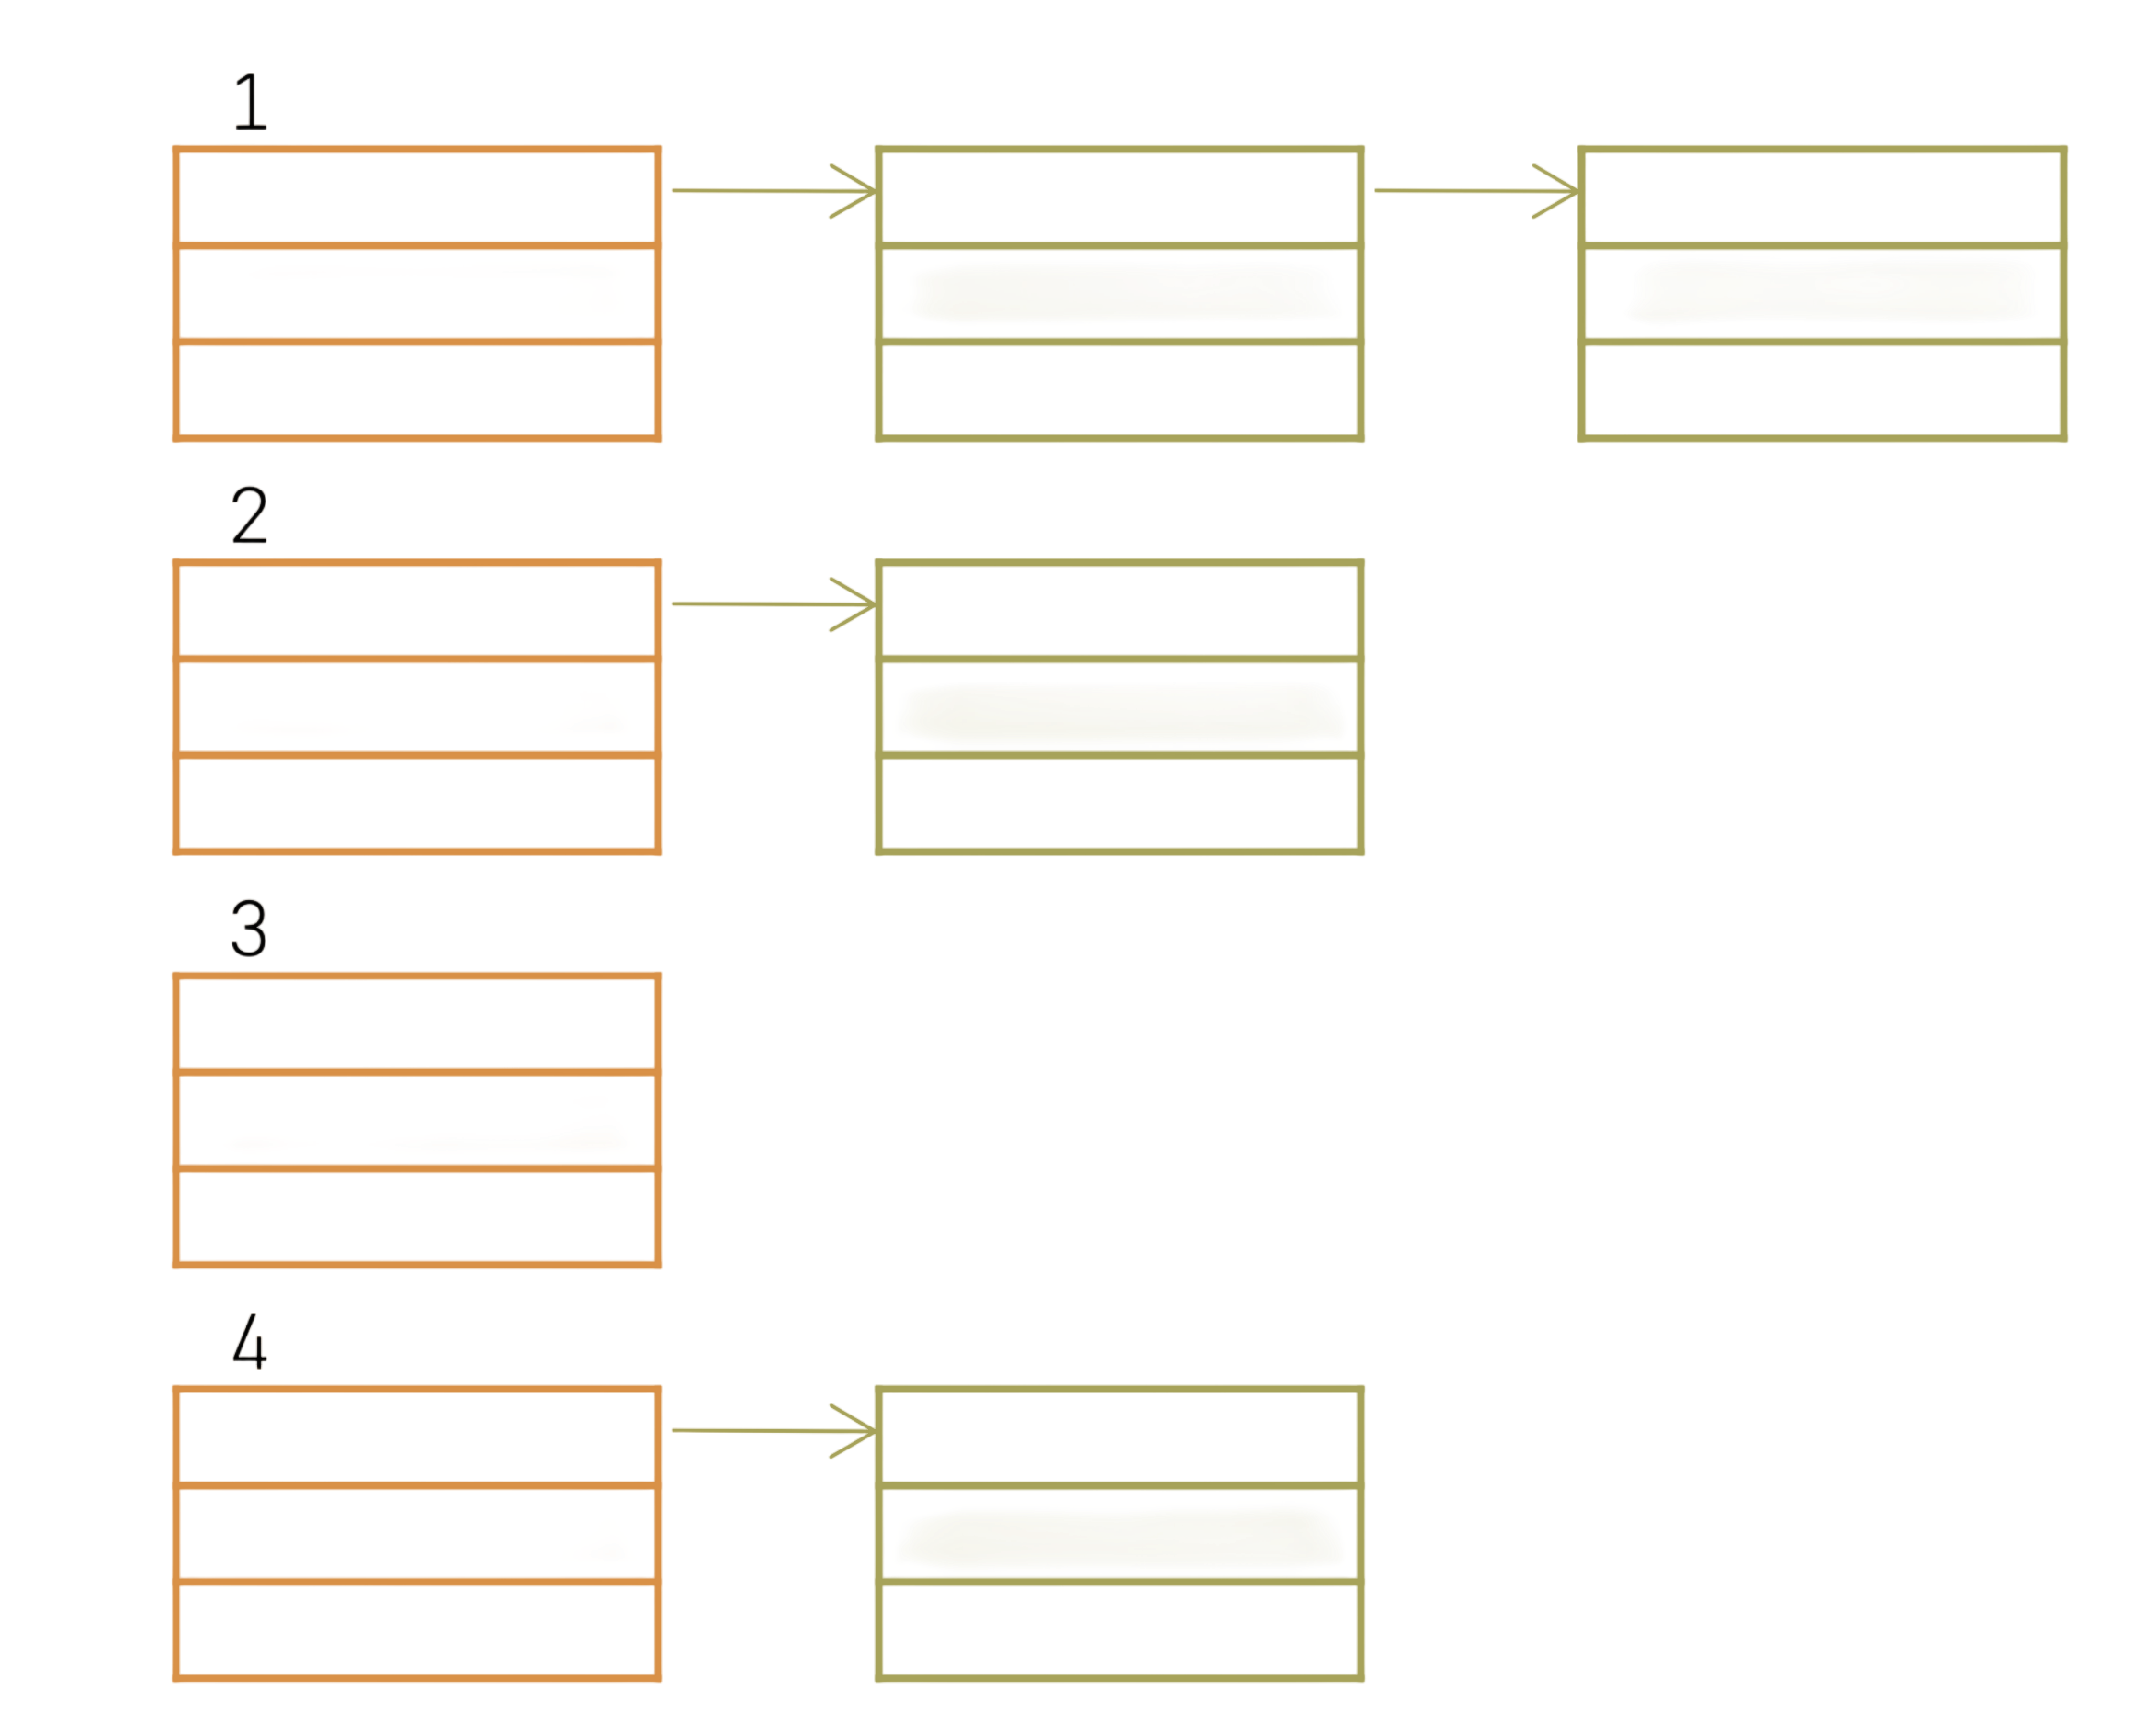
\includegraphics[width=0.5\textwidth]{images/gestione-collisioni-tabella-hash.png}
\end{figure}